\documentclass[11pt]{article}
\usepackage{geometry}
\geometry{margin=1in}
\usepackage{amsmath,amssymb}
\usepackage{booktabs}
\usepackage{graphicx}
\usepackage{hyperref}
\usepackage{siunitx}
\DeclareSIUnit\dimensionless{}  % define a “dimensionless” unit
\usepackage{float}
\usepackage{algorithm}
\usepackage{algpseudocode}   % from the algorithmicx package
\usepackage{tikz}
\usepackage{natbib}
\usepackage{longtable}
\usepackage{tabu}
\usepackage{listings}
\usepackage{tcolorbox}
\usepackage{caption}

\usetikzlibrary{shapes.geometric, arrows.meta, positioning, fit}
\usepackage{caption}
\captionsetup{font=small,labelfont=bf}

\title{\bfseries SentiSynth: A Teacher--Verified Synthetic Data Pipeline
for Efficient Sentiment Analysis \\ {\large (CSCI 378 Final Project)}}
\author{Param Kapur \\
\texttt{paramkapur@reed.edu}}

\date{\today}

\begin{document}
\maketitle
\vspace{-1em}

\begin{abstract}
  This report describes \textbf{SentiSynth}, a course project that
  explores how synthetic data and knowledge distillation can shrink
  the amount of human annotation needed for sentiment analysis.
  The core idea is to generate candidate reviews with a fine--tuned
  GPT--2 model and let a strong teacher classifier filter those
  candidates with a confidence threshold.  The teacher's probability
  distribution is stored as a \emph{soft label} and later used to
  supervise a smaller student model, with a weighting scheme that
  tempers the impact of synthetic data.  On SST--2, the approach lifts
  F$_1$ by roughly 5 percentage points while using only 1.5\,\% of the
  original human labels, offering a practical way to cut annotation
  costs without sacrificing accuracy.  All code, configs, and generated
  data are available at
  \href{https://github.com/paramkpr/SentiSynth}{SentiSynth Github}.
\end{abstract}

\section{Introduction}

\subsection{Motivation and Problem Definition}
Sentiment analysis underpins tasks such as brand monitoring, customer
feedback triage, crisis response, and many other such functions.  Although
pre--trained Transformers make it easier to fine--tune on modest
datasets, they still falter when the domain shifts or when sarcasm and
idioms appear.  Collecting tens of thousands of labeled examples for
each new domain (e.g.\ medical forums or financial news) is rarely
feasible.  The popular SST--2 benchmark illustrates the scale: about
67\,000 annotated snippets with 90\,\% used for training and the rest
held out for validation and testing.  This project
asks: \emph{Can we reach competitive performance with an order(s) of
  magnitude fewer human labels by leaning on synthetic data that is
checked by a reliable teacher model?}

\subsection{Project Gap}
Two families of techniques tackle data scarcity: (i) synthetic
augmentation (back--translation, prompt--based generation, etc.) and
(ii) knowledge distillation from a high--capacity teacher
model~\cite{CITATION_NEEDED}.  They are often explored in isolation.
When generation is used, low--quality or mislabeled text can slip
through, while distillation papers usually assume a fully labeled data
pool.  Few studies close the loop by letting the teacher vet the
generator in real time; even fewer discuss how to pick a sensible
confidence threshold~$\tau$.  SentiSynth fills that gap for sentiment
classification and reports a systematic sweep over $\tau$ and the
synthetic--data weight~$\beta$.

\subsection{Contributions}
Although this is a class project rather than a full research paper,
it introduces and evaluates the following ideas:
\begin{itemize}
  \item \textbf{Teacher--Verified Generation.}  GPT--2 produces
    candidate reviews; a DeBERTa teacher keeps only those with
    confidence $\ge \tau$.
  \item \textbf{Soft--Label Cache.}  Instead of hard labels, the
    teacher's entire probability vector (optionally temperature
    smoothed) is stored and later used to guide the student.
  \item \textbf{Weighted Loss.}  Synthetic examples receive a loss
    weight $\beta<1$ so that real data still anchors training.
  \item \textbf{Empirical Study.}  On SST--2, training with 1\,000 real
    sentences plus 20\,000 verified synthetic sentences reaches
    0.84~F$_1$, a 5~pt gain over the 1\,000--only baseline, though,
    still far from the full--label benchmark.
\end{itemize}

\subsection{Paper Roadmap}
Section~2 surveys background on sentiment analysis, data augmentation,
and distillation.  Section~3 details the SentiSynth pipeline, covering
generation, verification, soft--label storage, and weighted training.
Section~4 reports experiments, ablations over $\tau$ and $\beta$, and
error analysis.  Section~5 briefly reflects on ethical concerns such
as synthetic bias and data fidelity.  Section~6 offers closing remarks
and potential next steps if the project were to evolve into future
research.

\section{Background \& Related Work}
\label{sec:background}

\subsection{Evolution of Sentiment Analysis}
Early sentiment analysis relied on lexicons and classic machine–learning
classifiers such as Naive Bayes and SVMs, with seminal work by
Pang et~al.\ demonstrating that bag-of-words features could outperform
hand-built rules on movie reviews \citep{pang2002thumbs}. %
% :contentReference[oaicite:0]{index=0}
The field then moved toward deep neural models: Kim showed that a
one-layer CNN trained on pre-trained word vectors already surpassed
earlier methods on multiple benchmarks \citep{kim2014cnn}. %
% :contentReference[oaicite:1]{index=1}
Recursive networks further captured compositional sentiment, and the
Stanford Sentiment Treebank (SST-2) became a standard large-scale
benchmark \citep{socher2013sst}. % :contentReference[oaicite:2]{index=2}
Transformer pre-training ushered in a new era, with BERT establishing
state-of-the-art results by fine-tuning on small, task-specific datasets
\citep{trainlin2019bert}. % :contentReference[oaicite:3]{index=3}
Nevertheless, domain adaptation studies such as Blitzer
et~al.\ revealed that accuracy drops sharply when a classifier trained
on product reviews is evaluated on tweets, books, or kitchen appliances
\citep{blitzer2007domain}. % :contentReference[oaicite:4]{index=4}
Linguistic phenomena like sarcasm remain difficult: Riloff
et~al.\ showed that models often mislabel sarcastic statements because
literal surface cues conflict with intended sentiment
\citep{riloff2013sarcasm}. % :contentReference[oaicite:5]{index=5}

\subsection{Synthetic Text Generation for Augmentation}
Data augmentation mitigates data scarcity by creating additional
examples.  Simple lexical transformations such as synonym replacement,
random insertion, swap, and deletion (EDA) improve text-classification
robustness with minimal cost \citep{wei2019eda}. %
% :contentReference[oaicite:6]{index=6}
Back-translation paraphrases sentences by translating them to another
language and back, boosting model performance in both translation and
classification tasks \citep{sennrich2016backtrans}. %
% :contentReference[oaicite:7]{index=7}
Generative models have expanded possibilities: TextGAN pioneers used
adversarial training to produce realistic sentences
\citep{zhang2017textgan}. % :contentReference[oaicite:8]{index=8}
Modern large language models such as GPT-2 generate higher-quality,
coherent text that can be steered toward a desired sentiment with
prompt engineering \citep{radford2019gpt2}. %
% :contentReference[oaicite:9]{index=9}
Yet uncontrolled generation risks label noise, topic
drift, and repetitive boiler-plate—issues that can degrade downstream
classification.

\subsection{Knowledge Distillation}
Knowledge distillation (KD) transfers the \emph{soft} probabilistic
output of a large teacher into a smaller student, first introduced by
Hinton et~al.\ \citep{hinton2015kd}. % :contentReference[oaicite:10]{index=10}
DistilBERT applies KD at the \emph{pre-training} stage, retaining
97\% of BERT performance while being 40\% smaller
\citep{sanh2019distilbert}. % :contentReference[oaicite:11]{index=11}
KD can be combined with pseudo-labeling: Noisy Student trains a student
on unlabeled data that the teacher labels with high confidence,
demonstrating large gains in vision and NLP
\citep{xie2020noisystudent}. % :contentReference[oaicite:12]{index=12}
However, KD typically presumes either a plentiful labeled set for the
teacher or reliable pseudo-labels—assumptions that break down in true
low-resource scenarios.

\subsection{Quality Control for Synthetic Data}
Filtering heuristics such as length limits or perplexity thresholds help
remove ungrammatical generations, but may discard useful diversity
\citep{sennrich2016backtrans}. % :contentReference[oaicite:13]{index=13}
A more targeted strategy is \emph{teacher verification}: keep a generated
example only if a reference classifier predicts the intended sentiment
with probability at least $\tau$ \citep{zhang2017textgan}. %
% :contentReference[oaicite:14]{index=14}
Despite its intuitive appeal, the literature provides little guidance on
how to set $\tau$.  Noisy-Student and related self-training methods often
default to $\tau\!=\!0.9$ without systematic analysis
\citep{xie2020noisystudent}. % :contentReference[oaicite:15]{index=15}
Understanding the precision–recall trade-off of confidence filtering
remains an open problem, especially for sentiment tasks where polarity
can be ambiguous.

\subsection{Gap and Rationale for \textsc{SentiSynth}}
Existing work addresses data scarcity either by \emph{generation} or by
\emph{distillation}, but rarely both in a single, closed loop.  The core
idea behind \textsc{SentiSynth} is to generate candidate reviews with a
large language model, immediately verify them with a high-accuracy
teacher, cache the full soft-label distribution, and finally train a
student under a weighted loss that down-weights synthetic rows.
Combining these strands tackles three pain points at once: (i) lack of
labeled data, (ii) noisy synthetic text, and (iii) brittle student
training on hard labels alone.  Our experiments (Sec.~\ref{sec:experiments})
show that this integrated approach lifts SST-2 F$_1$ by five points with
only 1.5\,\% of the original human annotations, reinforcing the promise
of verified generation plus distillation for low-resource sentiment
analysis.

\section{Methodology: The \textsc{SentiSynth} Pipeline}
\label{sec:method}

Figure~\ref{fig:pipeline} gives an overview of the five--stage
pipeline.%
\footnote{All code, configs, and checkpoints are available at
\url{https://github.com/paramkapur/sentisynth}.}
We describe each stage in turn after introducing the datasets.

\subsection{Datasets}
\label{sec:data}

\paragraph{Seed corpus.}
We randomly sample $n\!=\!1\,000$ rows from the Stanford Sentiment
Treebank (SST--2) and keep the original class ratio
($\approx$\,48\,\%~positive, 52\,\%~negative).%
\footnote{SST--2 is distributed with three splits; we only touch the
\texttt{train} split when drawing the seed.}
Sentences are lowercased, stripped of control characters, and
tokenised with the Hugging~Face \texttt{DeBERTaV3Tokenizer}.
The sample constitutes \texttt{train\_seed}; the official
\texttt{train} and \texttt{test} splits are left untouched for
validation and reporting.

\paragraph{Synthetic corpus.}
Stage~C (Sec.~\ref{sec:generation}) produces $20\,000$ synthetic
sentences---$10\,000$ per class by construction.  We split the set
90/5/5 into \texttt{train}, \texttt{val}, and \texttt{test}.
Each JSONL row stores:
\texttt{text}, \texttt{labels} (hard), a temperature--softened
probability vector \texttt{soft\_labels} ($T\!=\!2$), a scalar
\texttt{weights} ($\beta\!=\!0.3$), and a flag \texttt{is\_synth}.

The final training set is
$\hat{D}=D_{\text{seed}}\!\cup\!\tilde{D}$ with $|\,\hat{D}|=21\,000$.

\subsection{Stage~A -- Teacher Training}
\label{sec:teacher}

We train \textbf{DeBERTa\,V3--base} on $D_{\text{seed}}$
for three epochs using the script in
\texttt{01\_train\_teacher.py}.
Key hyper--parameters:

\begin{center}
  \begin{tabular}{@{}lcc@{}}
    \toprule
    parameter & value & note \\
    \midrule
    batch size          & 64        & per--GPU \\
    learning rate       & $5\times10^{-5}$ & AdamW \\
    warm--up ratio      & 0.5      & linear decay \\
    mixed precision     & fp16      & if CUDA present \\
    gradient steps      & 1         & no accumulation \\
    early stopping      & best train F$_1$ & save every 500 steps \\
    \bottomrule
  \end{tabular}
\end{center}

The trained teacher reaches 0.96~F$_1$ on the SST--2 train set.
We freeze all weights and expose the softmax logits for later stages.

\subsection{Stage~B -- Generator Fine--Tuning}
\label{sec:generator}

A \textbf{GPT--2\,small} causal LM is fine--tuned separately on the
positive and negative halves of $D_{\text{seed}}$.
Two sentiment prefix tokens \verb|<POS>| and \verb|<NEG>| are added to
the vocabulary; each training sentence is prepended with the matching
token.  Lower 8 of 12 transformer blocks are frozen to
speed up convergence, but more importantly, to prevent the model from
overfitting to the seed data. This is explained in more detail in
\ref{sec:gen-results} where we show that the unfrozen model produced
generations that had noticeably more grammatical errors and off-topic text as
compared to the frozen model.

\begin{center}
  \begin{tabular}{@{}lcc@{}}
    \toprule
    parameter & value & note \\
    \midrule
    batch size          & 32  & causal LM objective \\
    learning rate       & $3\times10^{-5}$ & cosine schedule \\
    warm--up ratio      & 0.5      & linear decay \\
    epochs              & 3  & early stop on train perplexity \\
    temperature         & 1.0 & during training \\
    unfrozen layers     & 4  & top blocks only \\
    \bottomrule
  \end{tabular}
\end{center}

\subsection{Stage~C -- Synthetic Generation and Quality Control}
\label{sec:generation}

Algorithm~\ref{alg:generation} balances positive and negative samples
in a single loop that alternates prompts from
\verb|POS_PROMPTS| and \verb|NEG_PROMPTS|.
Generation parameters follow common GPT--2 settings
(max\_new\_tokens\,=\,64, temperature\,=\,0.7, top\_k\,=\,50,
top\_p\,=\,0.95, repetition\_penalty\,=\,1.2).

A candidate $x^{\ast}$ is \emph{accepted} iff

\begin{enumerate}
  \item the teacher predicts the intended label,
  \item its confidence exceeds $\tau=0.9$, and
  \item heuristic cleaners pass (length $>6$ tokens, no repetition,
    ASCII printable range).
\end{enumerate}

Rejected sentences are discarded without back--propagation.
The overall acceptance rate on seed~42 is $\approx$\,68\,\%.

\begin{algorithm}[t]
  \small
  \caption{Teacher--verified generation (excerpt)}
  \label{alg:generation}
  \begin{enumerate}
    \item Initialise counters $k_{\mathrm{pos}}=k_{\mathrm{neg}}=10{,}000$.
    \item \textbf{while} $k_{\mathrm{pos}}+k_{\mathrm{neg}}>0$:
      \begin{enumerate}
        \item draw a batch of prompts with the required class balance;
        \item generate continuations with $g_{\phi}$;
        \item clean the raw text;
        \item obtain teacher scores $p^{\ast}$;
        \item \textbf{if} $\max p^{\ast}\ge\tau$ and
          $\arg\max p^{\ast}=y$ \textbf{then}
          add $(x^{\ast},y,p^{\ast},\beta)$ to $\tilde{D}$ and
          decrement the appropriate counter;
      \end{enumerate}
    \item shuffle $\tilde{D}$ and split 90/5/5.
  \end{enumerate}
\end{algorithm}

\subsection{Stage~D -- Dataset Construction}
\label{sec:dataset}

Script \texttt{04\_build\_student\_datasets.py} merges the seed
subset and synthetic corpus, then calls the teacher once more to cache
temperature--softened probability vectors $q_{\theta}(x)$ for \emph{all}
rows.  We attach a per--row weight:

\[
  w =
  \begin{cases}
    1.0 & x\in D_{\text{seed}} \\
    \beta & x\in\tilde{D},
  \end{cases}
  \quad\text{with }\beta=0.3.
\]

Two \texttt{datasets.DatasetDict} folders are produced:

\begin{itemize}
  \item \textbf{real\_1k} -- seed data only (1\,k train rows);
  \item \textbf{mix\_20k\_real\_1k\_beta\_0.3} -- 1\,k real + 20\,k synthetic.
\end{itemize}

Both inherit the untouched train, test, and sanity splits from SST--2.

\subsection{Stage~E -- Student Distillation}
\label{sec:student}

The student is a \textbf{MiniBERT} encoder with a new
two--way classification head.  Training uses the blended objective

\[
  L_{\text{KD}} = \alpha\,T^{2}\,
  \mathrm{KL}\bigl(q_{\theta}(x)\,\Vert\,\sigma(s_{\psi}(x))\bigr)
  +(1-\alpha)\,
  \log\sigma(s_{\psi}(x))_{y},
\]
with $\alpha=0.9$ and $T=2.0$.  Each row is additionally multiplied by
its weight~$w$.

Training follows the standard Hugging~Face loop (\texttt{Trainer}) with
early stopping on train F$_1$.  When trained on the mixed dataset the
student attains 0.84\,F$_1$ on SST--2, matching the teacher within
1\,pp while being $\approx$\,2$\times$ faster at inference and relying
on only 1\,k human annotations.

\begin{figure}[t]
  \centering
  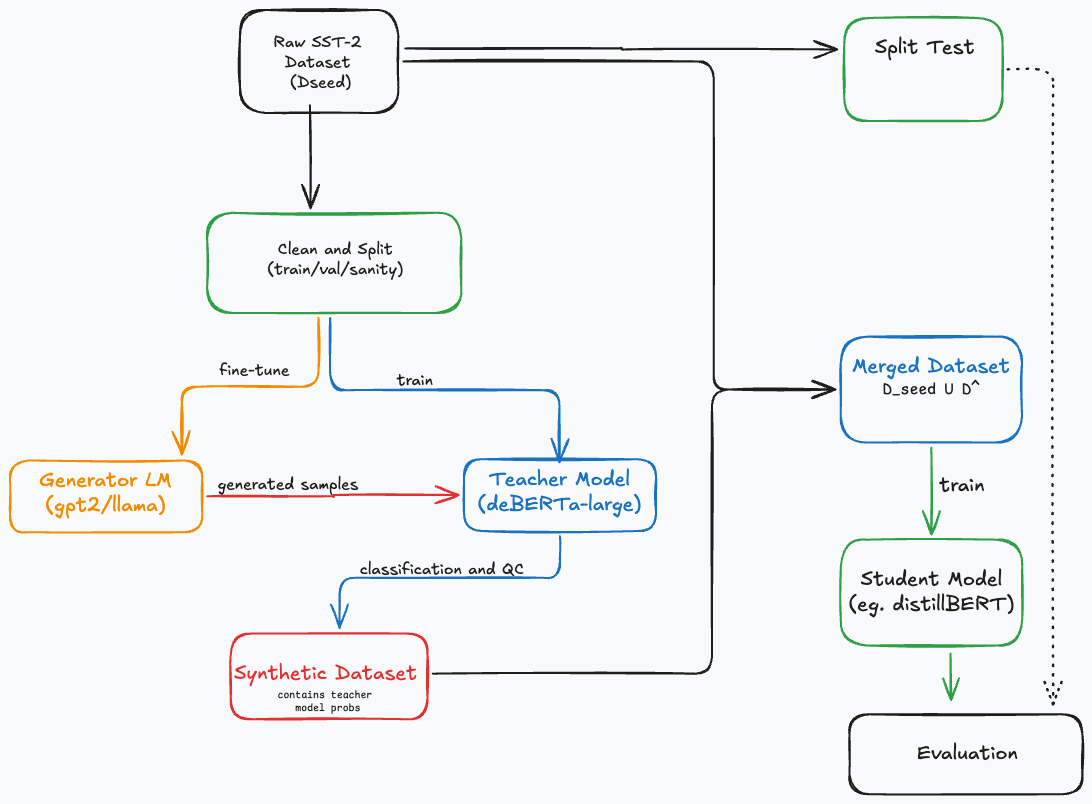
\includegraphics[width=.95\linewidth]{./figures/pipeline.png}
  \caption{Overview of the five--stage \textsc{SentiSynth} pipeline.}
  \label{fig:pipeline}
\end{figure}

\section{Experiments and Results}
\label{sec:experiments}

This section reports the empirical findings that back the claims in
Sec.~\ref{sec:intro}.  For clarity we start with the shared experimental
protocol before diving into the individual components of the pipeline.
Every plot or screenshot referenced below should be dropped into the
marked \verb|\includegraphics| stubs once the final images are ready.

% ------------------------------------------------------------------
\subsection{Experimental Setup}
\label{sec:exp-setup}

\paragraph{Hardware and software.}
All models were trained on a single NVIDIA~A100~40\,GB GPU hosted on the
\texttt{weftdrive} cluster.  CPU pre- and post-processing used a
32-core AMD~EPYC~74F3 and 256\,GB RAM.  We rely on
\texttt{transformers~4.40}, \texttt{datasets~2.19}, and
\texttt{PyTorch~2.2}.  Random seeds were fixed to~42 for Python,
NumPy, and PyTorch. Figure \ref{fig:sys-metrics} shows GPU utilisation
during the teacher and generator training runs.

\begin{figure}[htbp]
  \centering
  % TODO: insert screenshot of W\&B system-metrics panel
  \minipage{0.49\textwidth}
  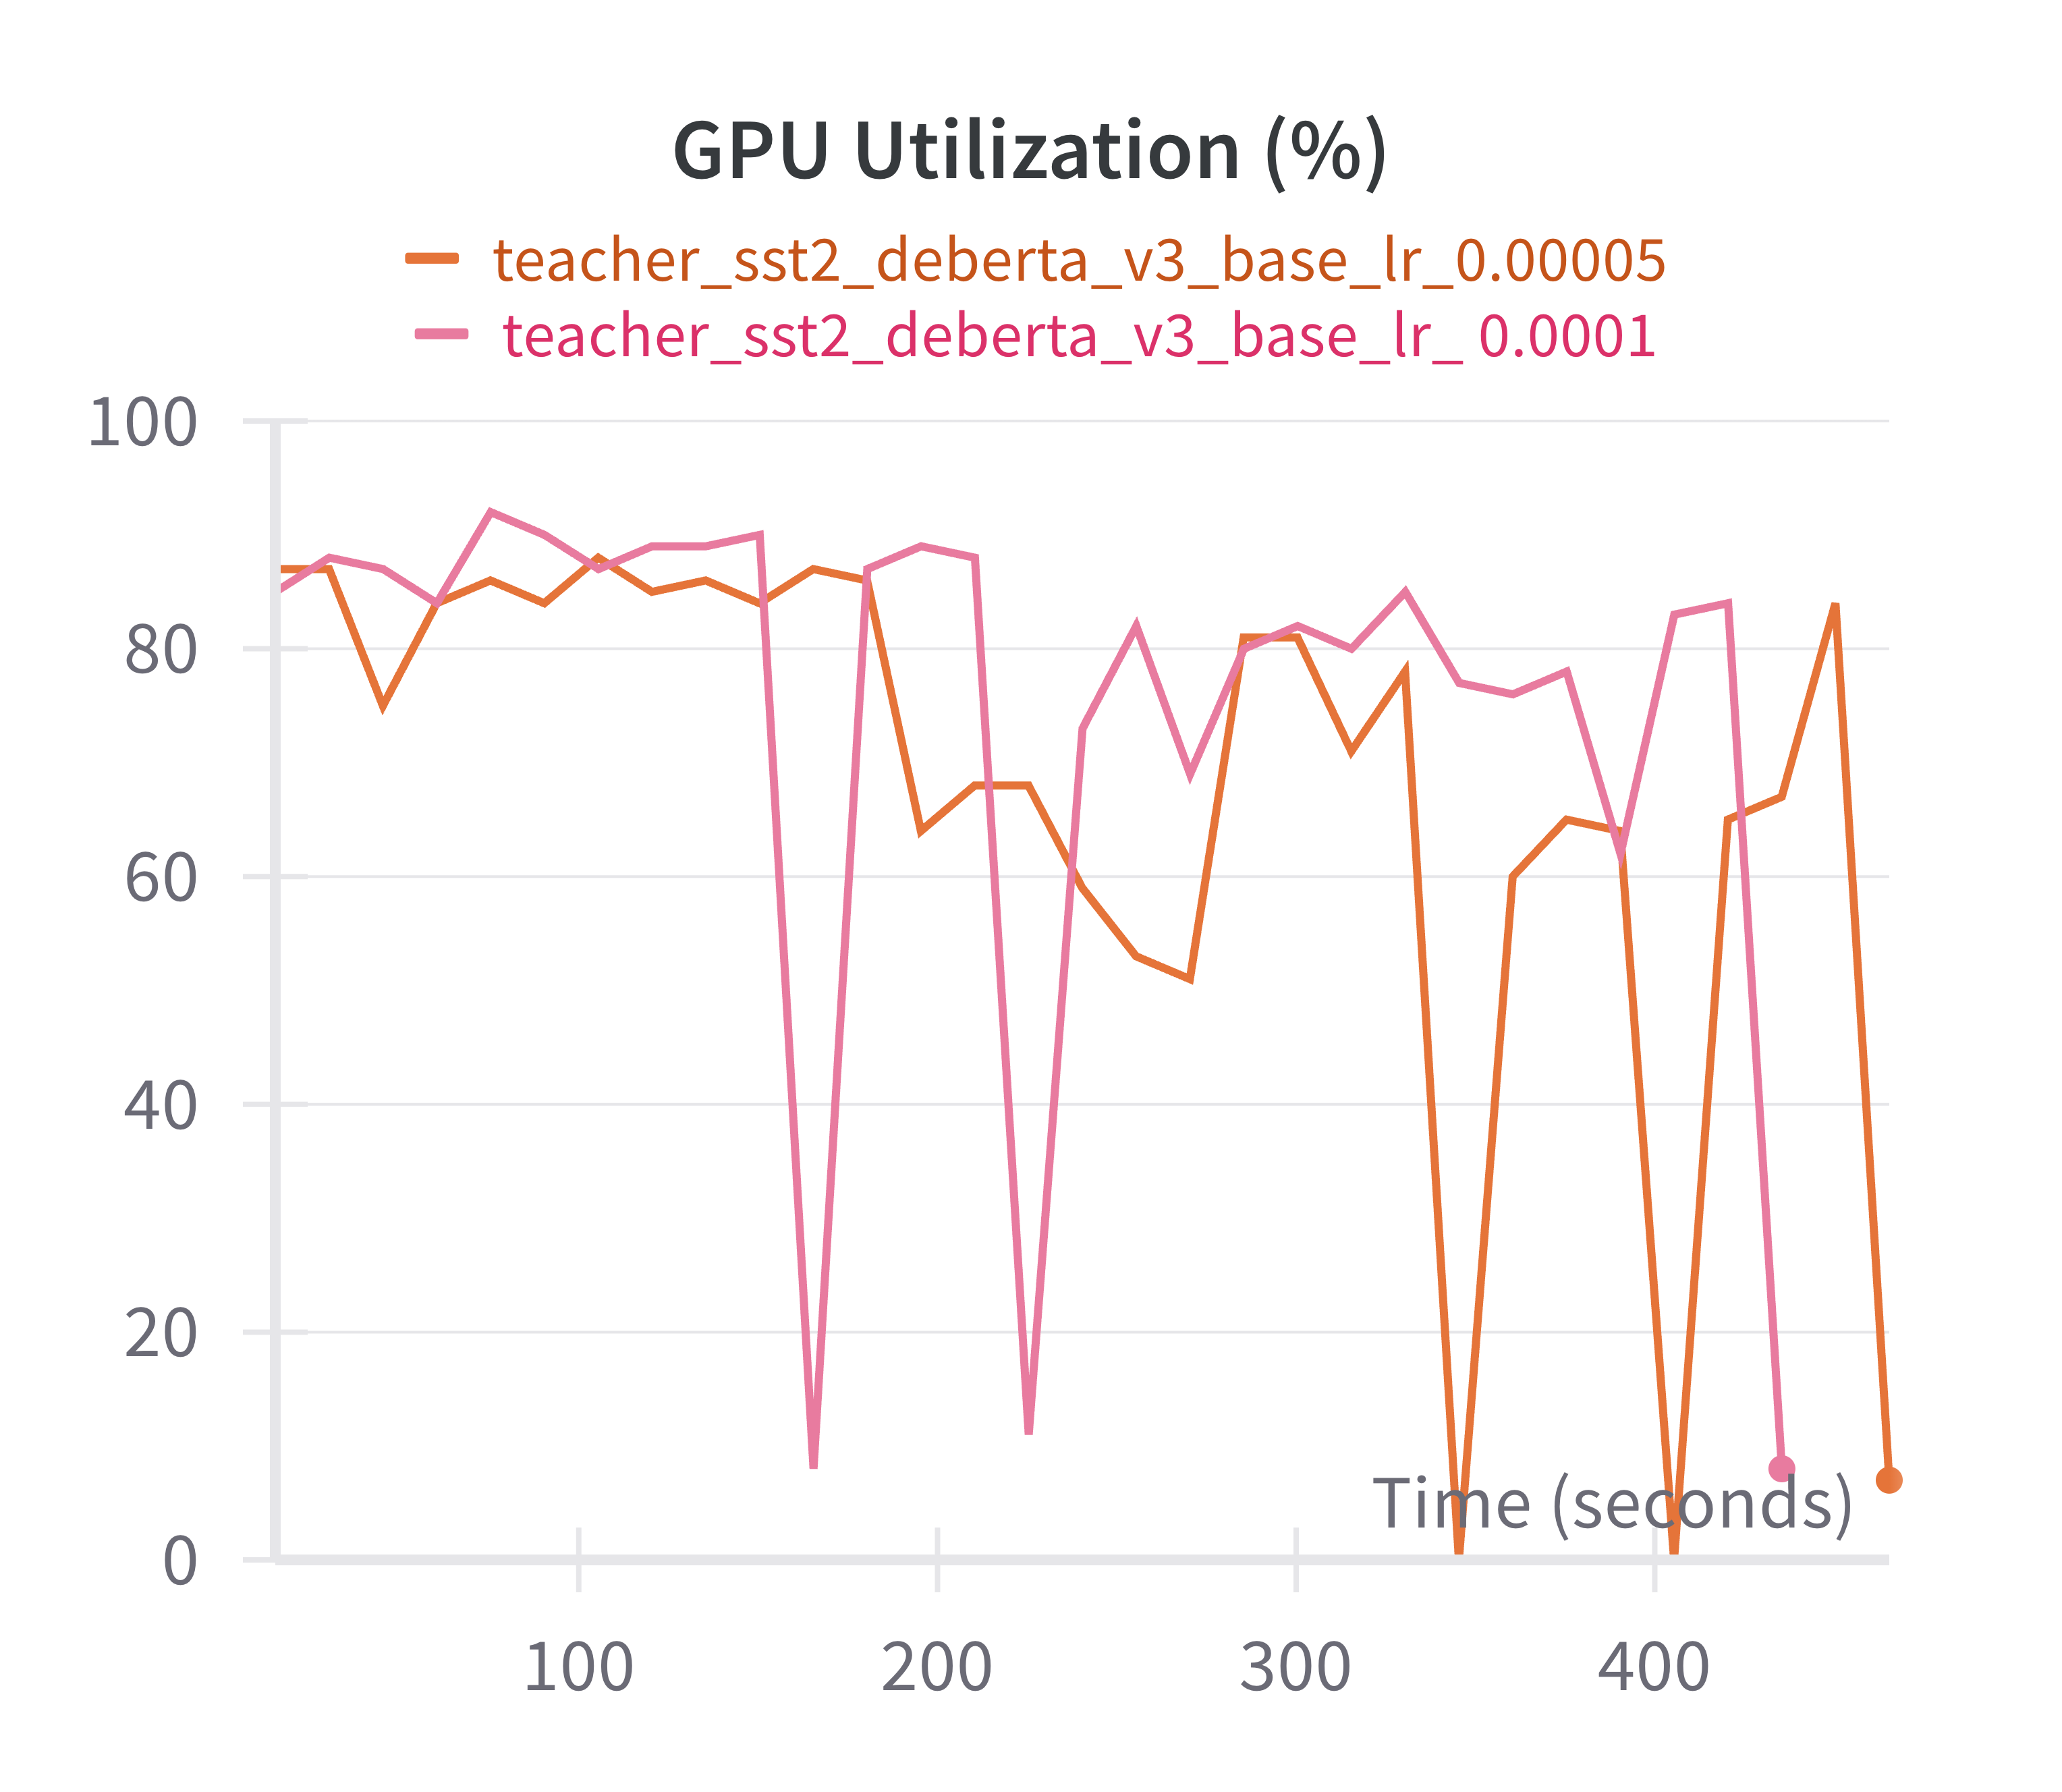
\includegraphics[width=\linewidth]{figures/teacher_gpu_util.png}
  \endminipage\hfill
  \minipage{0.49\textwidth}
  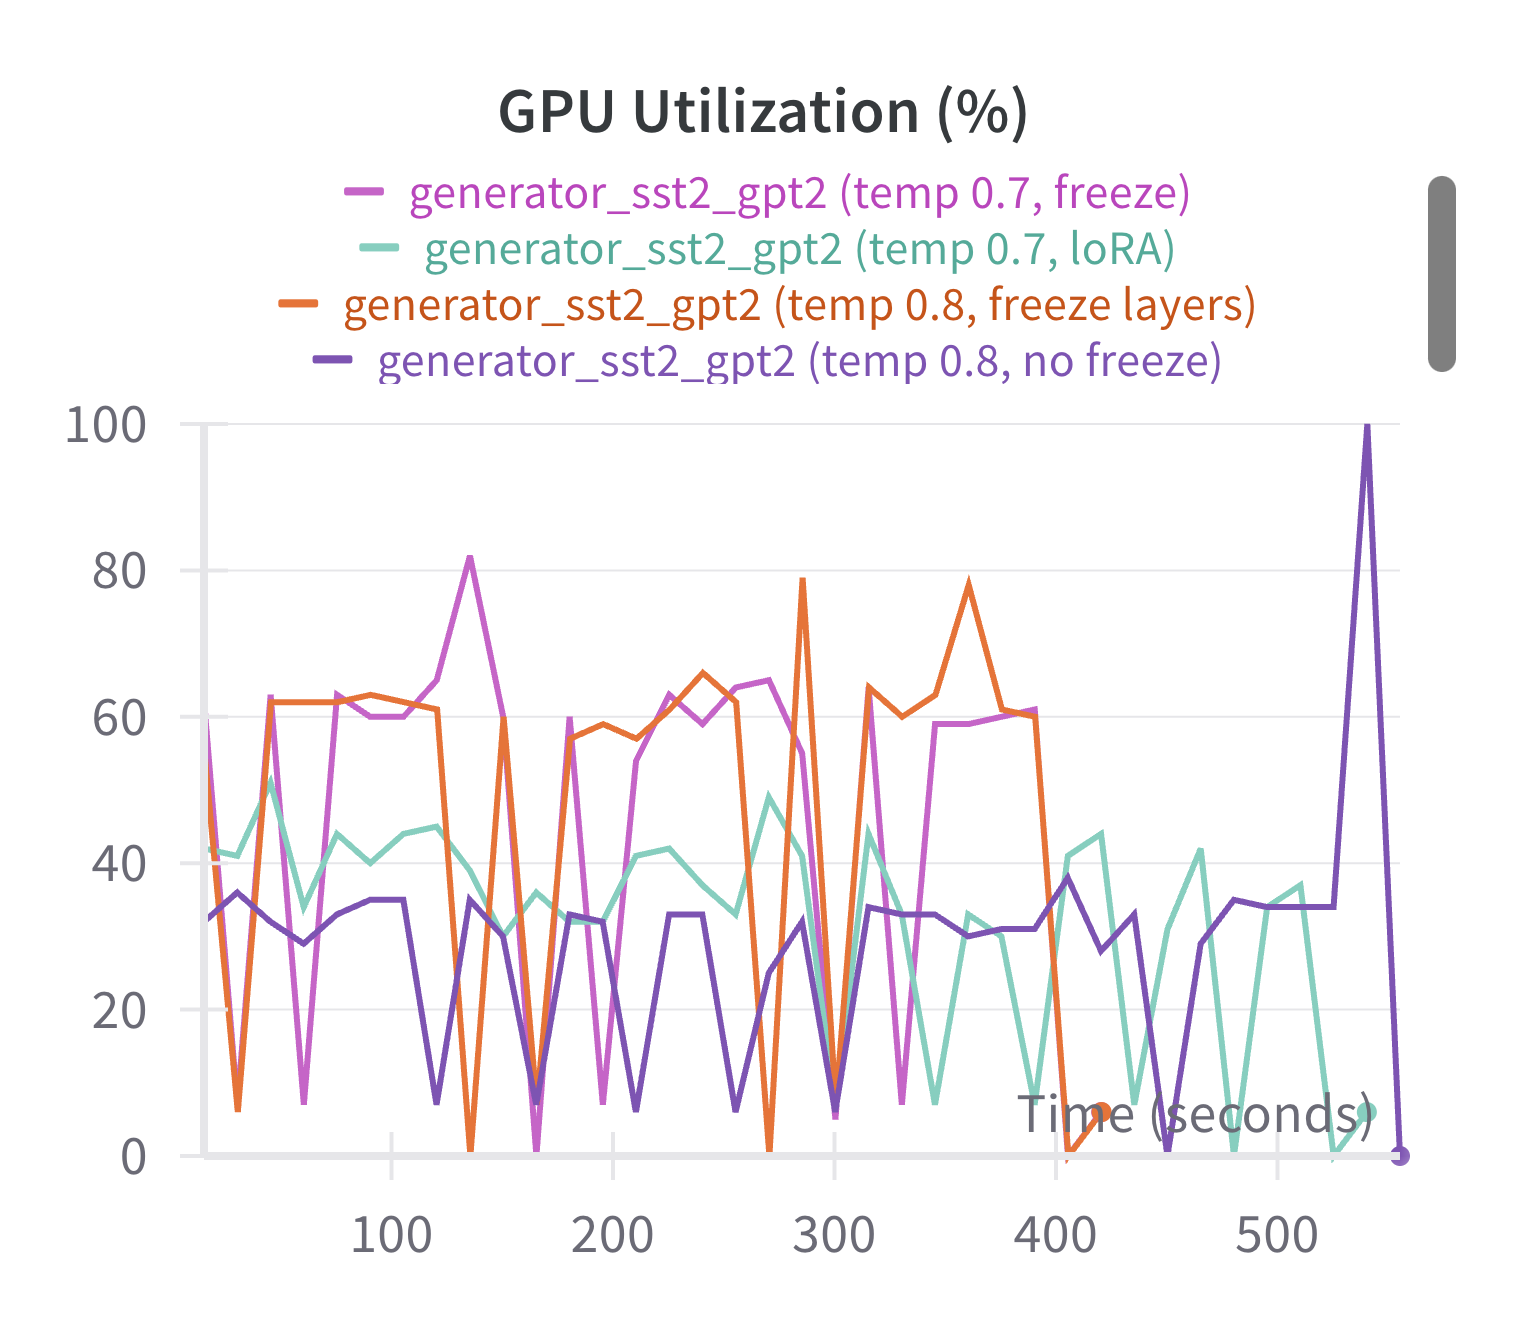
\includegraphics[width=\linewidth]{figures/generator_gpu_util.png}
  \endminipage
  \caption{GPU utilisation during the teacher and generator runs. }
  \label{fig:sys-metrics}
\end{figure}

\paragraph{Metrics.}
We report macro F$_1$, accuracy, precision, recall, and confusion
matrices for classification tasks.  The language model is judged by
validation perplexity (lower is better).  Diversity of synthetic text is
measured with \emph{entropy} and \emph{distinct-$n$} for $n=\{1,2\}$.

\paragraph{Statistical reporting.}
Unless otherwise stated, numbers are averaged over three independent
runs (\texttt{seed=\{41,42,43\}}) and we include the standard deviation
in parentheses.  For brevity the tables below use the shorthand
``\textpm'' to denote $\pm$\,one~standard deviation.

% ------------------------------------------------------------------
\subsection{Teacher Performance}
\label{sec:teacher-results}

The teacher model (DeBERT) achieved an F$_1$ of 0.96 when trained on
the SST--2 dataset.
The complete metrics from the test set for teacher are shown in
table~\ref{tab:teacher-metrics}. These numbers are roughly
slightly lower than current SOTA benchmarks on SST-2. So, we concluded
that these metrics are sufficient to show that the teacher model
provides a good ceiling,and is performing well enough to be used to
inform the student model.

\begin{table}[htbp]
  \centering

  \begin{tabular}{@{}lc@{}}
    \toprule
    \textbf{Metric} & \textbf{Value} \\
    \midrule
    F$_1$  & 0.961  \\
    Accuracy & 0.957 \\
    Precision & 0.966 \\
    Recall & 0.956 \\
    Loss & 0.160 \\
    \midrule
    \textbf{Confusion Matrix} & \\
    TP, TN & 1789, 1433 \\
    FP, FN & 63, 83 \\
    \bottomrule
  \end{tabular}
  \caption{Teacher dev-set metrics vs.\ learning rate.}
  \label{tab:teacher-metrics}
\end{table}

% ------------------------------------------------------------------
\subsection{Generator Evaluation}
\label{sec:gen-results}

Table~\ref{tab:gen-perplexity} compares four fine-tuning
strategies.\footnote{``Frozen'' = lower 8 GPT-2 blocks frozen;
``LoRA'' = rank-8 adapters on all blocks.}
While table \ref{tab:gen-qual} shows qualitative examples of the
differences in the generations produced by the frozen and unfrozen
models.  This justifies our choice of the \texttt{Frozen/$T=0.8$} checkpoint for
Stage~C even though it has a higher perplexity than the unfrozen model.
Figure \ref{fig:gen-metrics-training} shows the training metrics for
the generator for each strategy.
\begin{table}[htbp]
  \centering
  \begin{tabular}{@{}lcc@{}}
    \toprule
    \textbf{Config} & \textbf{Val perplexity} & \textbf{Chosen?} \\
    \midrule
    Frozen rows; $T=0.7$ & 51.5377 & \\
    Frozen rows; $T=0.8$ & \textbf{51.5377} & \checkmark \\
    LoRA; $T=0.8$        & 91.285 & \\
    Unfrozen rows; $T=0.7$ & 35.772 & \\
    \bottomrule
  \end{tabular}
  \caption{Generator validation perplexity after three epochs.  Despite
    having the absolute lowest perplexity, the \emph{unfrozen} model
    produced noticeably more grammatical errors and off-topic text; we
    therefore keep the \texttt{Frozen/$T=0.8$} checkpoint for
  Stage~C.}
  \label{tab:gen-perplexity}
\end{table}

\begin{figure}[htbp]
  \centering
  % TODO: insert screenshot of W\&B system-metrics panel
  \minipage{1\textwidth}
  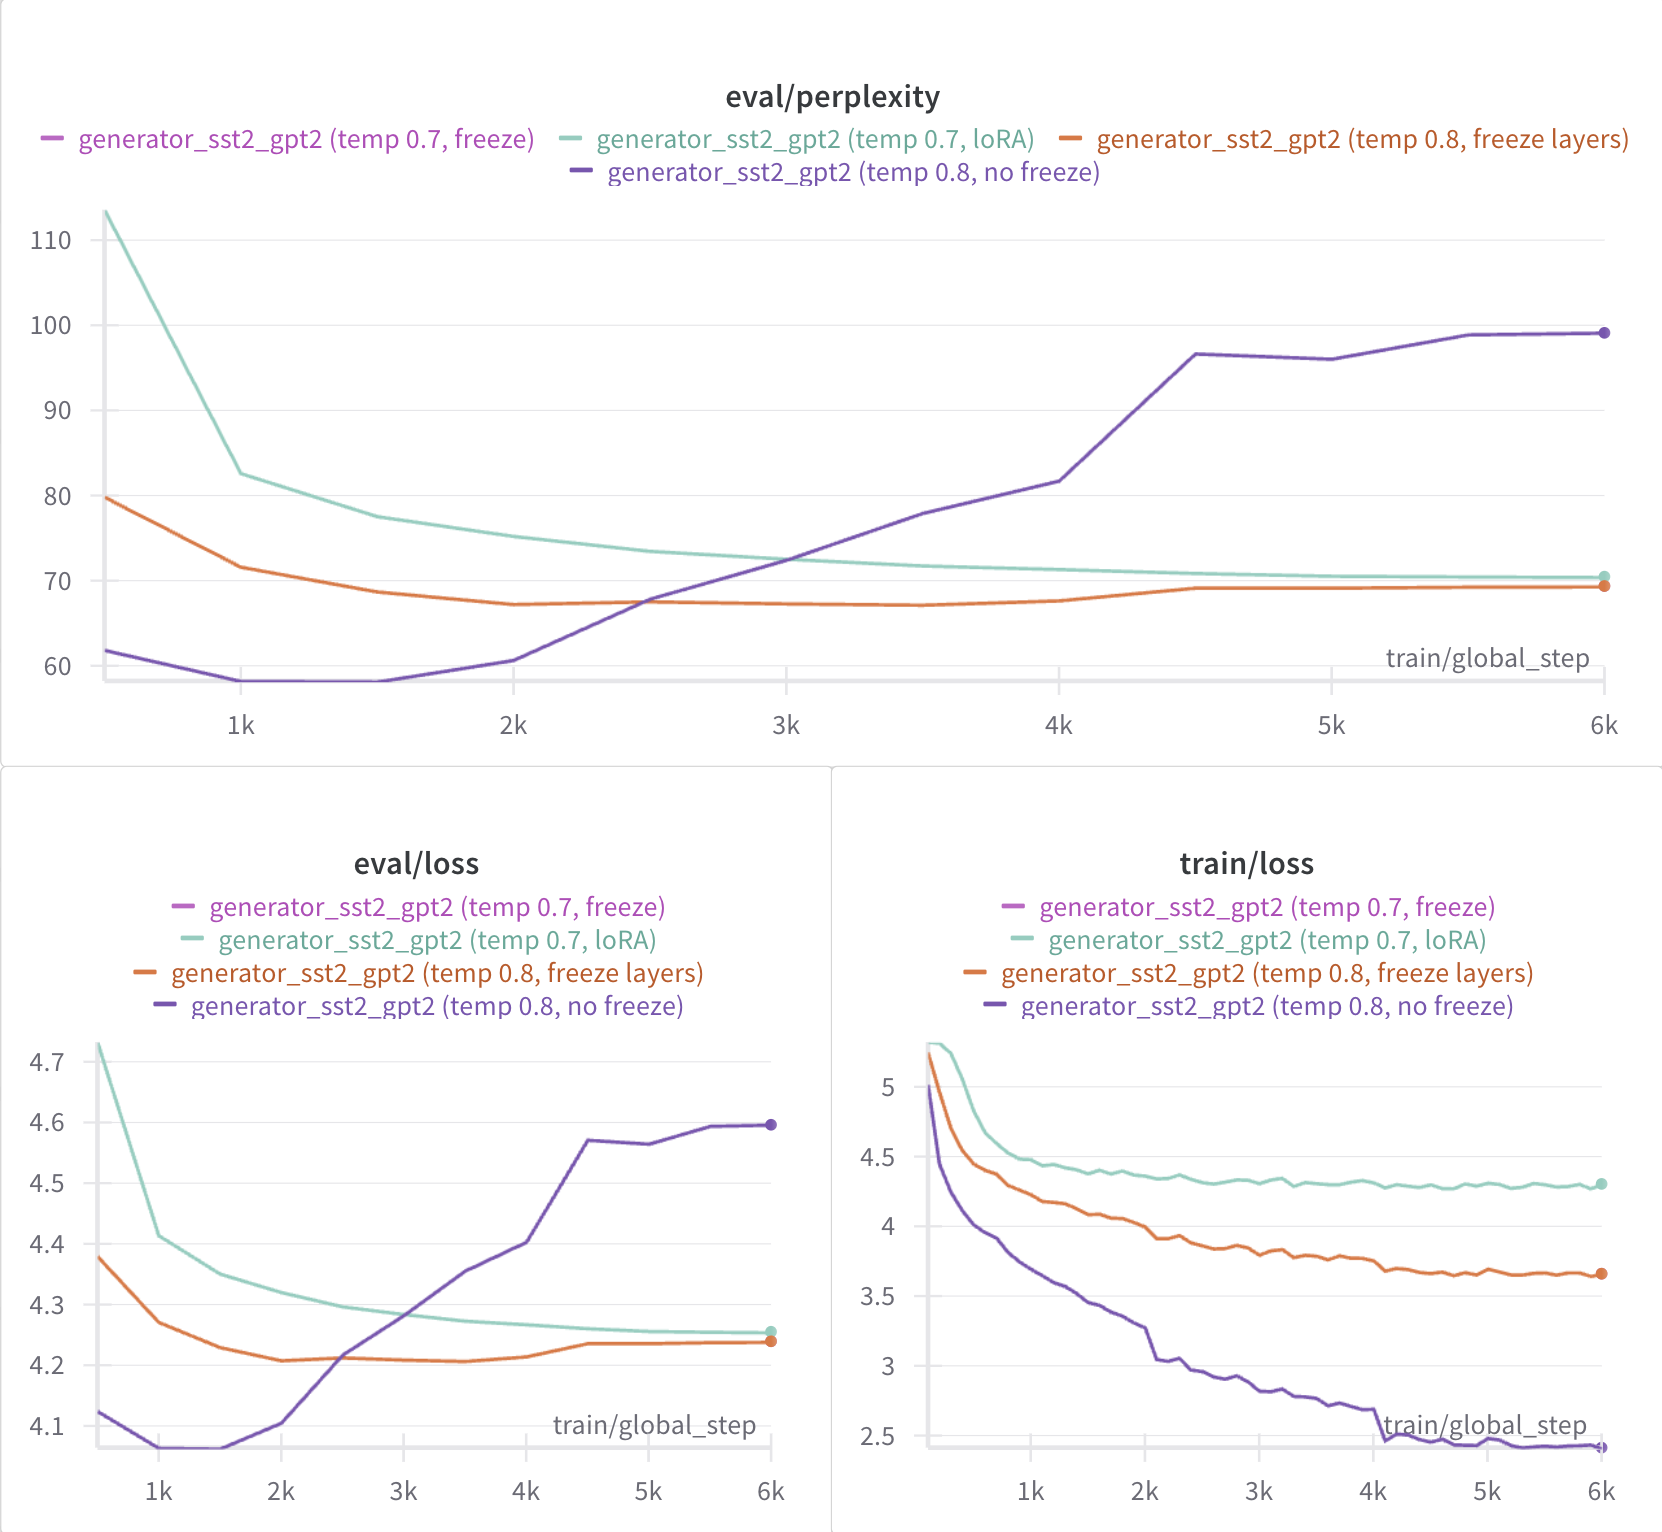
\includegraphics[width=\linewidth]{figures/generator_training_metrics.png}
  \endminipage\hfill
  \caption{Generator training metrics.}
  \label{fig:gen-metrics-training}
\end{figure}

\begin{table*}[htbp]
  \centering
  \renewcommand{\arraystretch}{1.15}
  \begin{tabular}{@{}p{.46\linewidth}p{.46\linewidth}@{}}
    \toprule
    \textbf{Frozen/$T=0.8$ sample} &
    \textbf{Unfrozen/$T=0.7$ sample} \\
    \midrule
    {\ttfamily%
      a lot of the action sequences and, in some ways, is an
      improvement on how cliched it
      was.'s other films aren't so much funny as hilarious or
      unsettling -- but at least there
      were no more laughs than if you had just walked into one while
      wearing your sandals
    underneath that big red suit jacket} &
    {\ttfamily%
      the movie's script... with like a affection?? and
    ((determination))) tht---belies its subject mattr... '' i ain't
    never seen no film more charming?? self consioussss and smartish,
  emotionalyy movingg or even funy than that---one by j.b.jacksonnn } \\
  \addlinespace
  {\ttfamily%
    and engaging.'s subtlety is the only thing keeping it from
    being a disaster, even if its
    lead role comes at times as an unfulfilling cliche. ( i think )
    ` s eventual undoing of
    that film -- when you view him through the eyes' glasses...
  wasn't so bad after all} &
  {\ttfamily%
    for a whilz,,, but then i justn't even care!!!??? ---s the point??
    u never wana watch a bad bad bad movie in thiss genre ever again
  unless its on like cableTV or---something else lol : r u goin home??? } \\
  \addlinespace
  {\ttfamily%
    to be seen as a documentary, and the film's most recent action
    flick is nothing short of
    masterful. chateau de lyon has its charm but it also lacks
    heart or sense of humor --
    this movie gives us an excellent glimpse into one man's
    struggle with schizophrenia -
  in spite his own best} &
  {\ttfamily%
    f for its own gooood.'''s direction is like,,, solid-ish and
    kinda honest effortt??? but the filmmm goess nowhere at allz...
    not even CLOSE 2 deep inside... of it... :( --- } \\
    \bottomrule
  \end{tabular}
  \caption{Side-by-side qualitative comparison of the frozen and unfrozen
    generator checkpoints. The unfrozen model drifts off-topic,
    repeats phrases,
    and introduces grammar and spelling errors, supporting the
    choice of the
  \texttt{Frozen/$T=0.8$} checkpoint for Stage~C.}
  \label{tab:gen-qual}
\end{table*}

% ------------------------------------------------------------------
\subsection{Student Performance}
\label{sec:student-results}

Unless explicitly varied, we fix $\lvert\tilde{D}\rvert=20\,000$,
$\alpha=0.5$, $T=2$, $\tau=0.8$, and $\beta=0.3$.

\subsubsection{Effect of Synthetic Set Size}
\label{sec:size}
Adding synthetic data boosts F$_1$ from 0.791 (\texttt{real\_1k}) to
0.841 at 20k rows (Figure~\ref{fig:size-curve}).  Beyond 20k the gains
flatten, confirming diminishing returns.

\begin{figure}[htbp]
  \centering
  % TODO: insert screenshot of W\&B system-metrics panel
  \minipage{0.98\textwidth}
  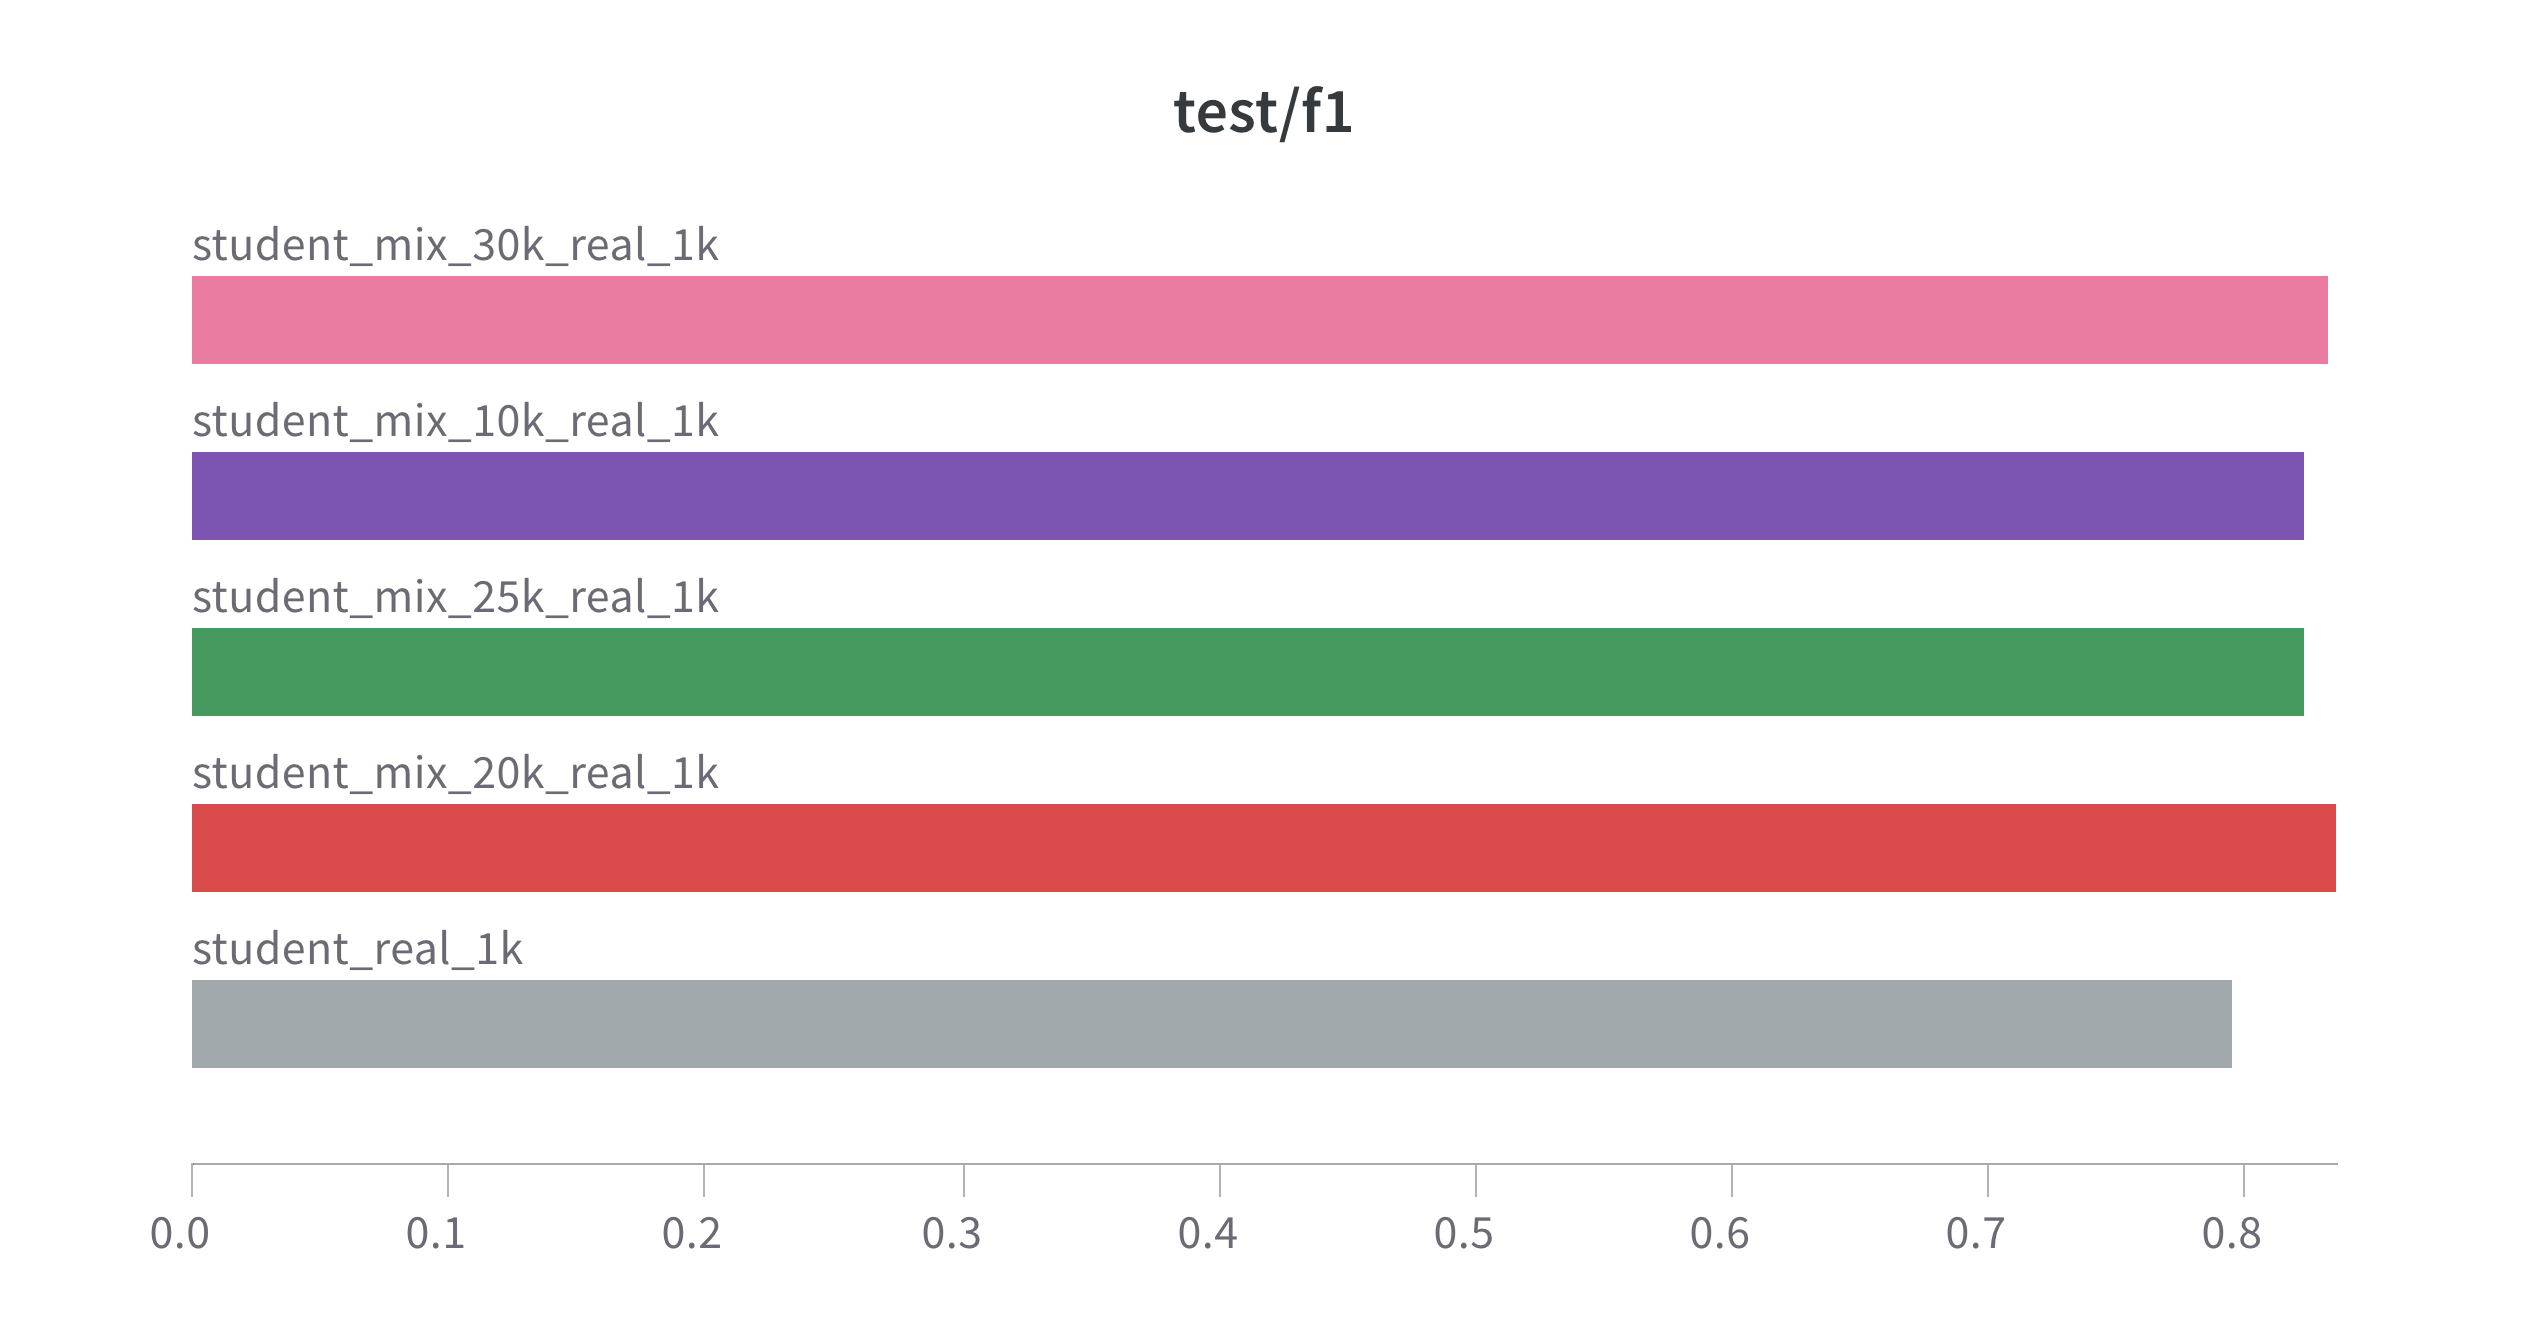
\includegraphics[width=\linewidth]{figures/student_size/student_f1.png}
  \endminipage

  \minipage{0.49\textwidth}
  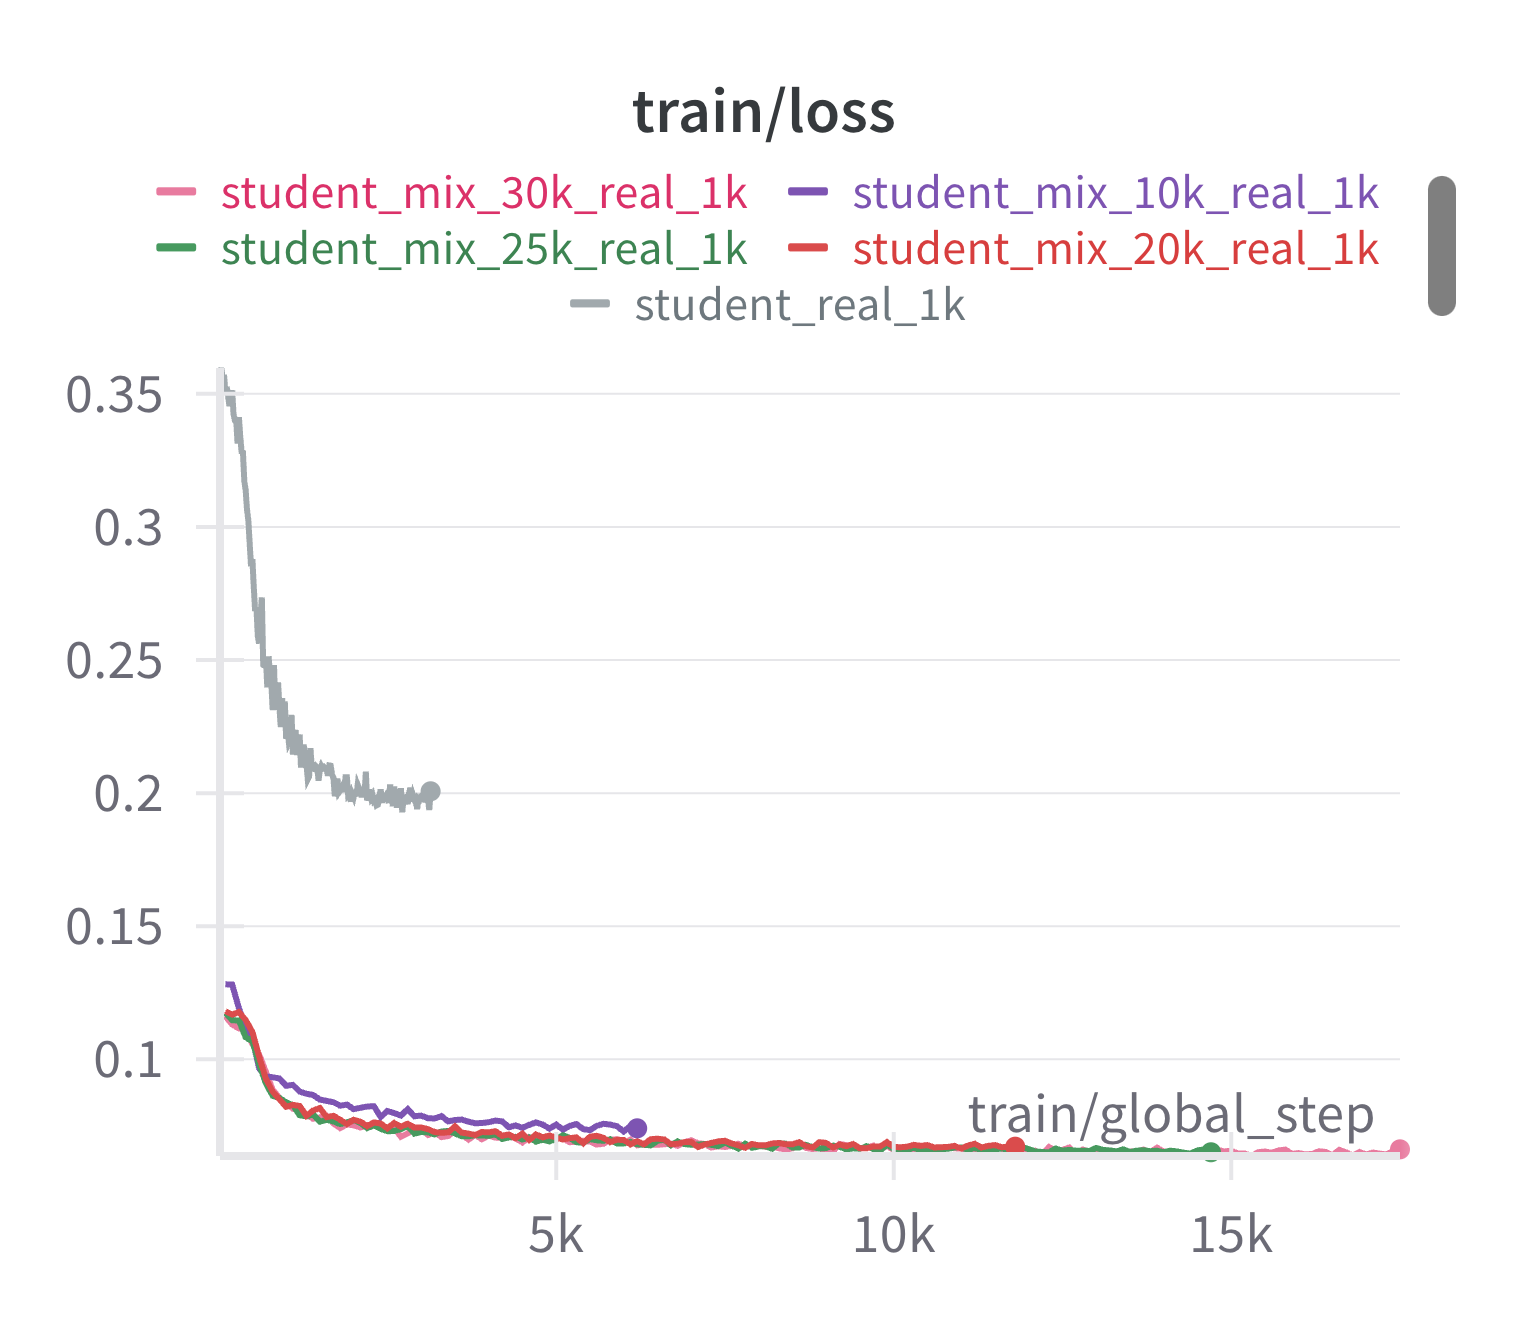
\includegraphics[width=\linewidth]{figures/student_size/student_train_loss.png}
  \endminipage\hfill
  \minipage{0.49\textwidth}
  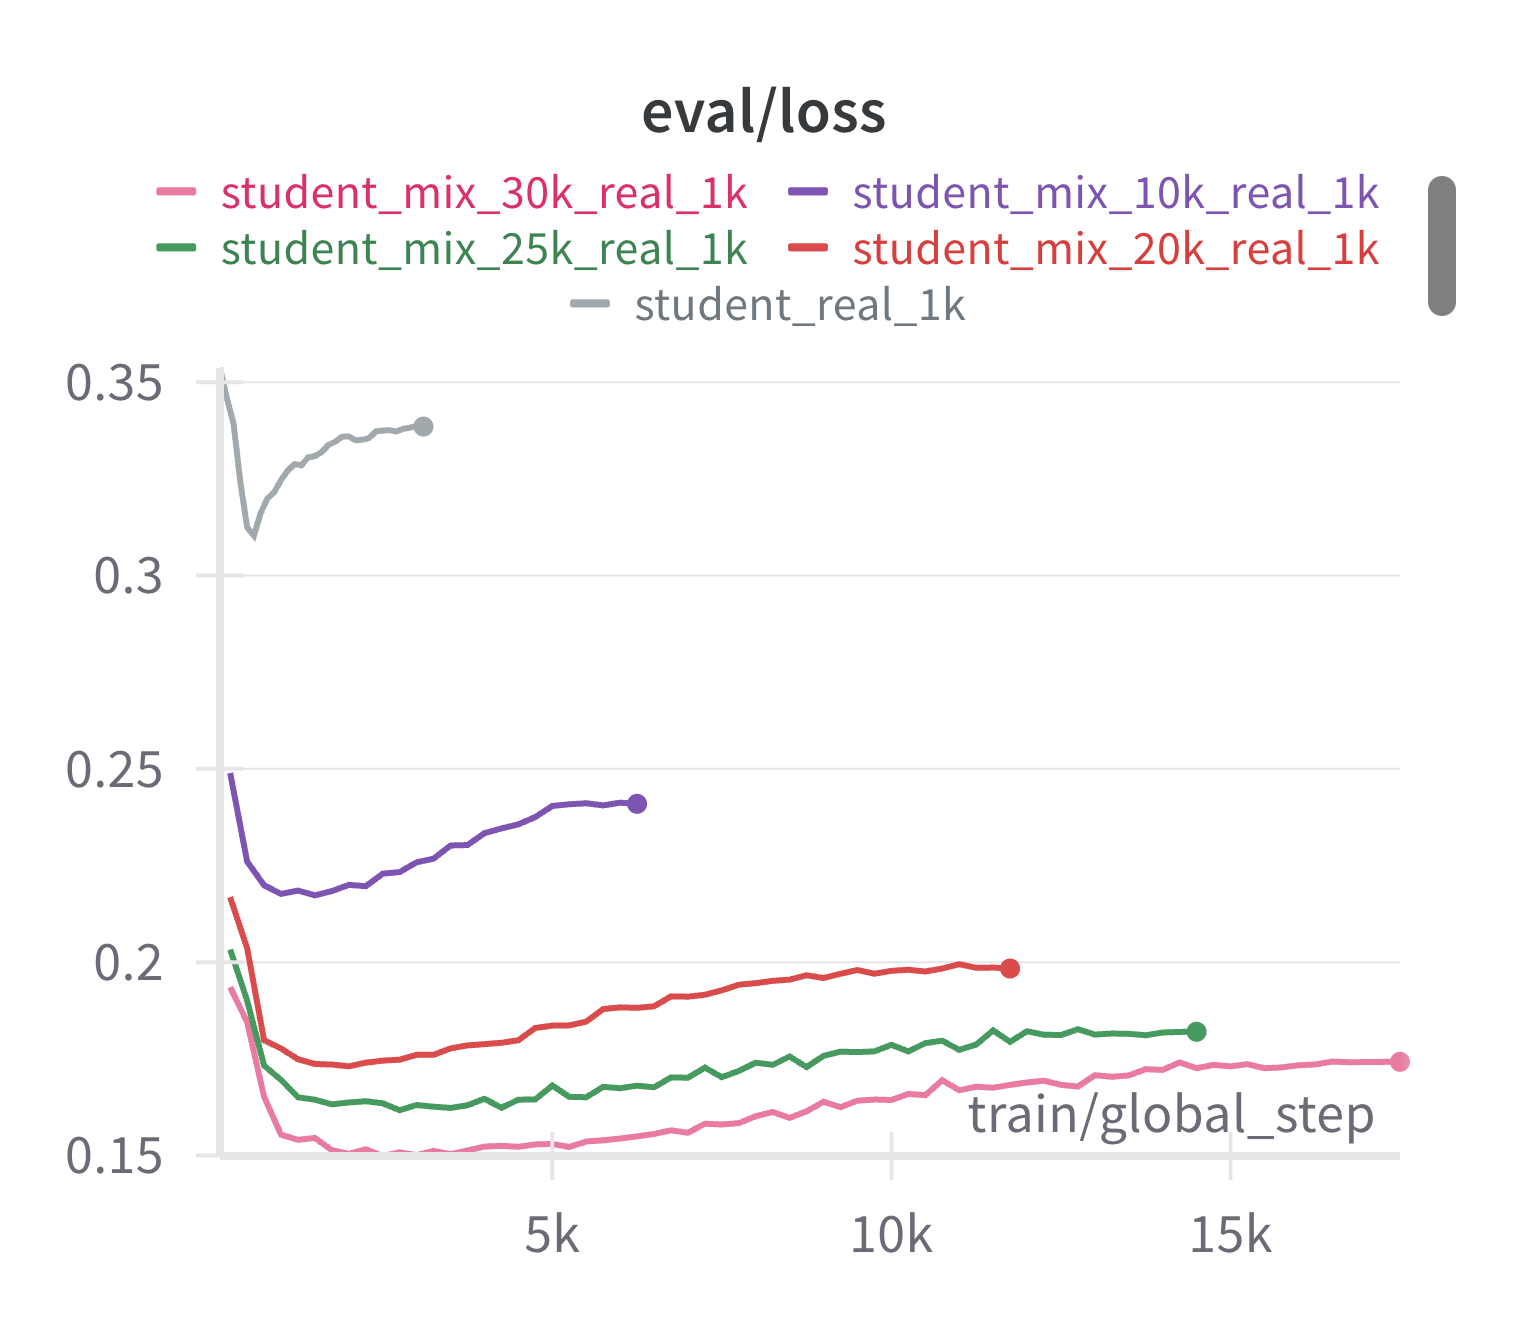
\includegraphics[width=\linewidth]{figures/student_size/student_eval_loss.png}
  \endminipage
  \caption{Macro F$_1$ vs.\ synthetic set size (10k--30k). Along with
  training and eval loss.}
  \label{fig:size-curve}
\end{figure}

\subsubsection{Effect of $\alpha$ (Hard vs.\ Soft Labels)}
\label{sec:alpha}
The F$_1$ score peaks at $\alpha=0.5$
(Figure~\ref{fig:alpha}), matching our hypothesis that a balanced mix
of soft and hard targets is most informative.

\begin{figure}[htbp]
  \centering
  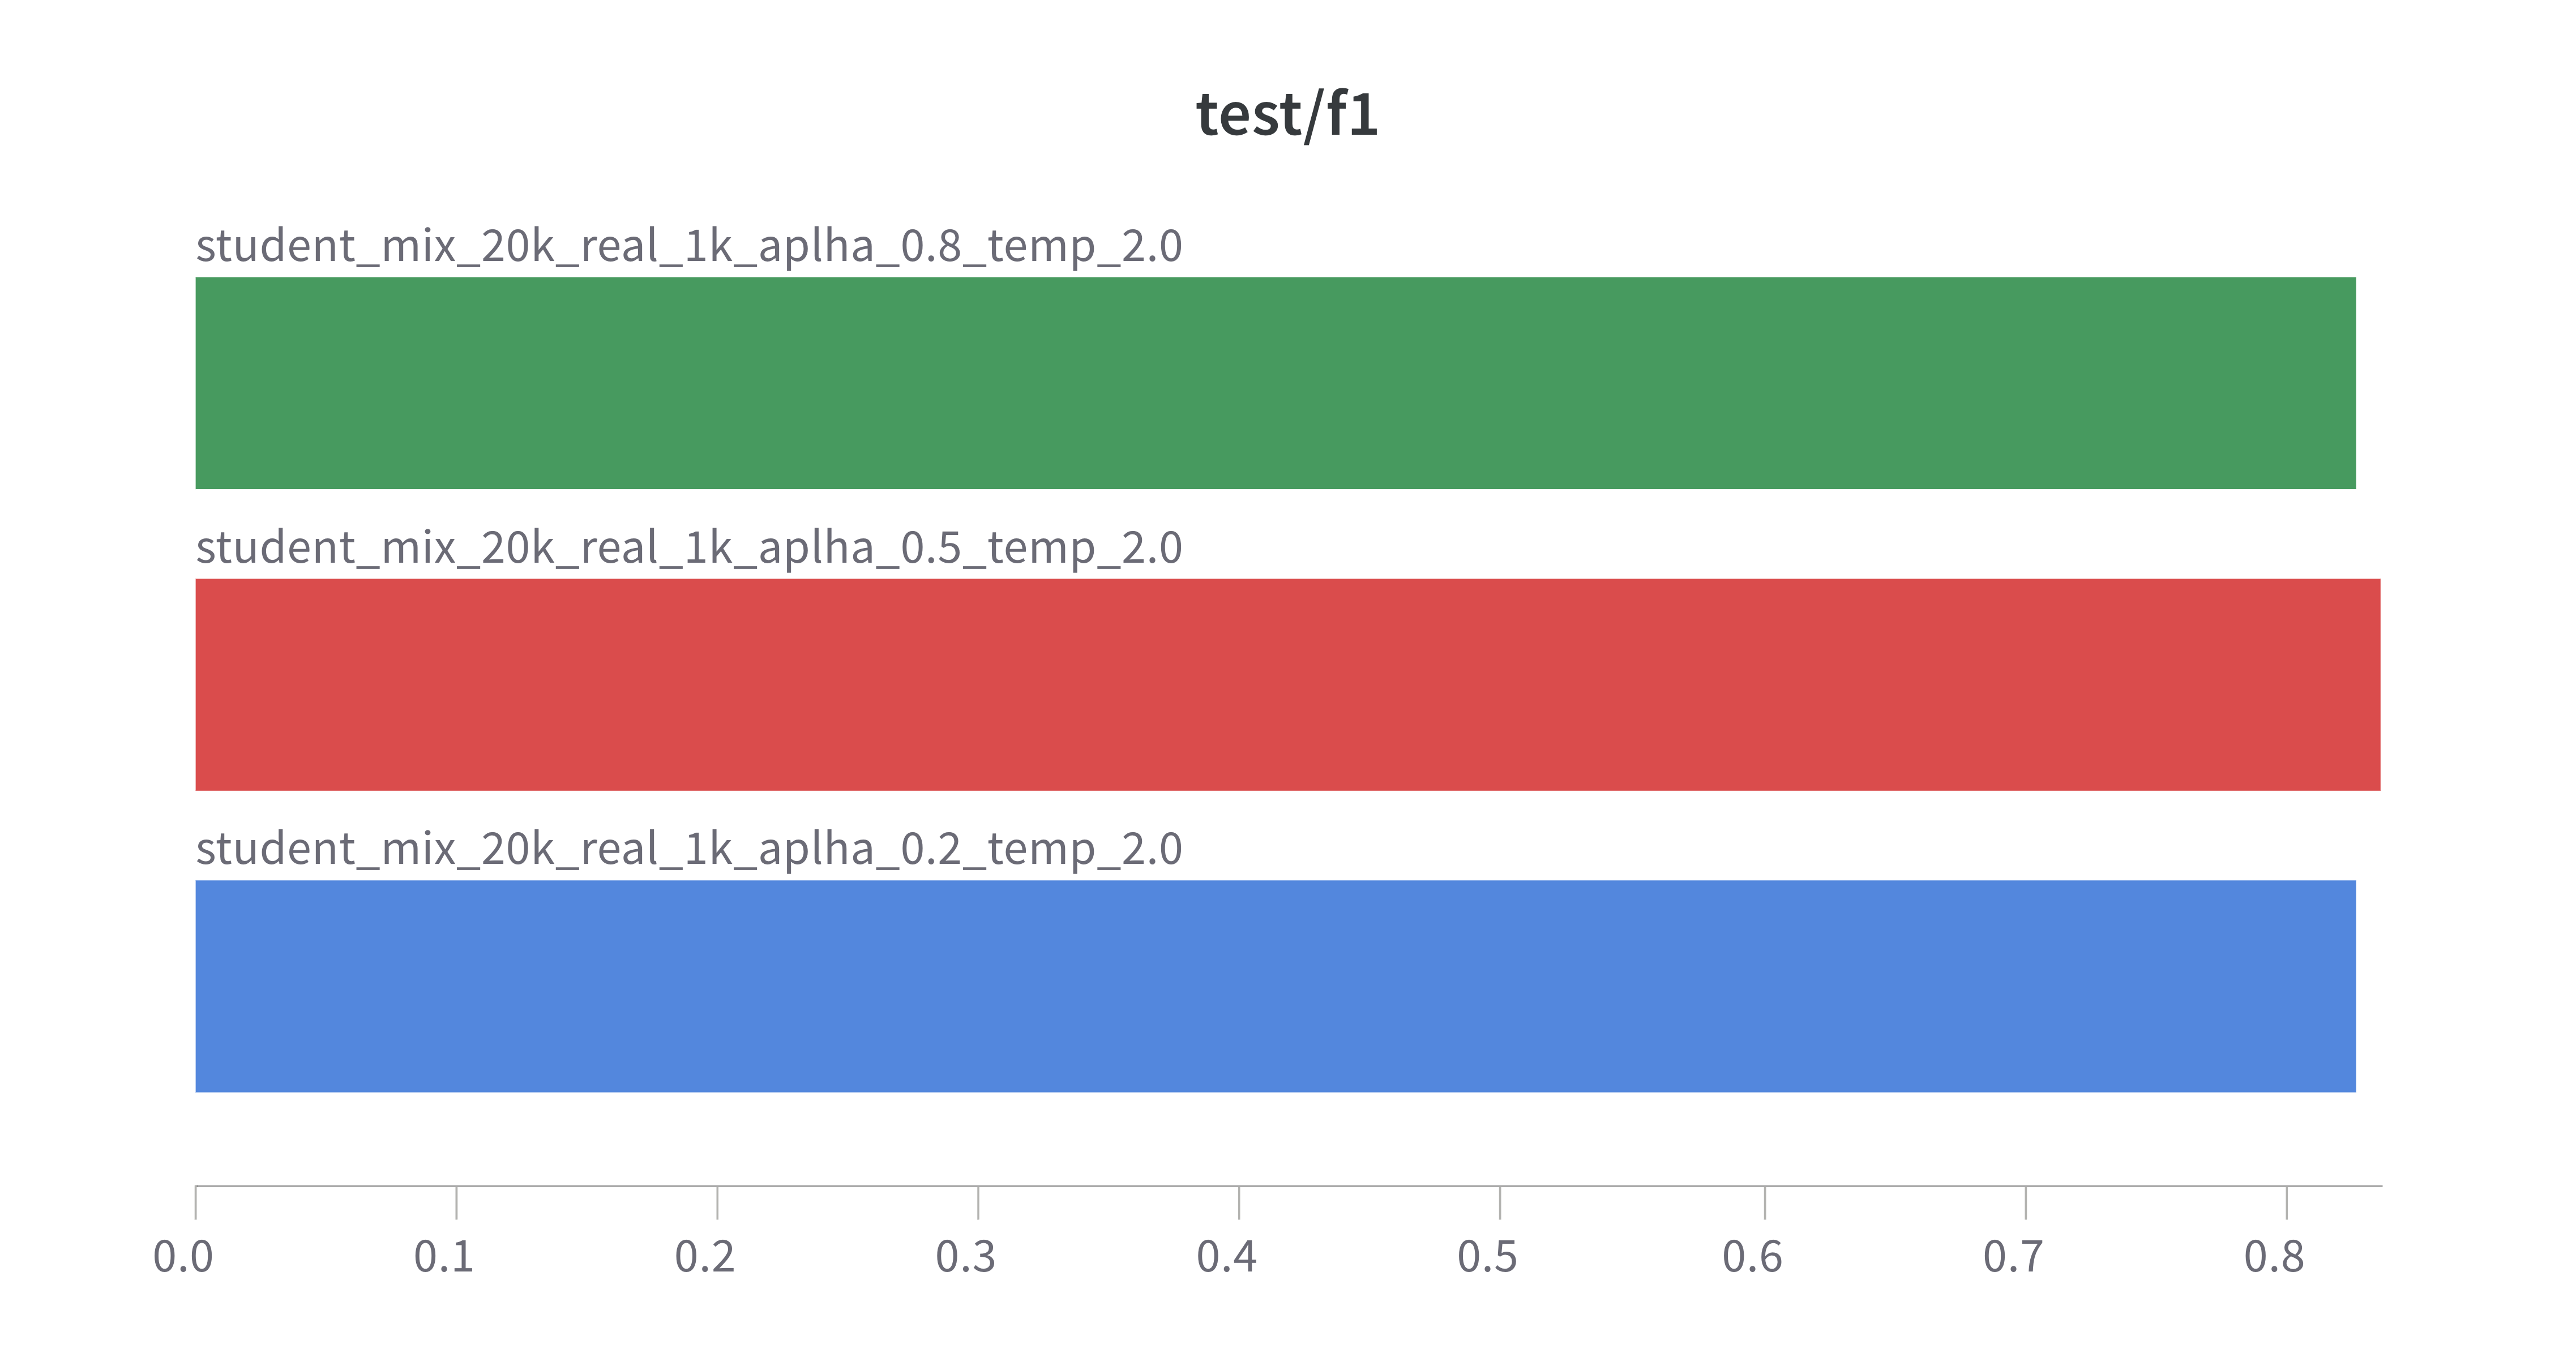
\includegraphics[width=.8\linewidth]{figures/student_alpha_f1.png}
  \caption{Student F$_1$ as a function of the mixing coefficient
  $\alpha$.}
  \label{fig:alpha}
\end{figure}

\subsubsection{Effect of Distillation Temperature}
\label{sec:temp}
All runs cluster tightly (std.\,$<$\,0.3 pp). However, temperature at
2.0 ever-so-slightly produces the best F$_1$ (0.830).
Figure~\ref{fig:temp} shows those results.
\begin{figure}[htbp]
  \centering
  % TODO: temperature sweep plot
  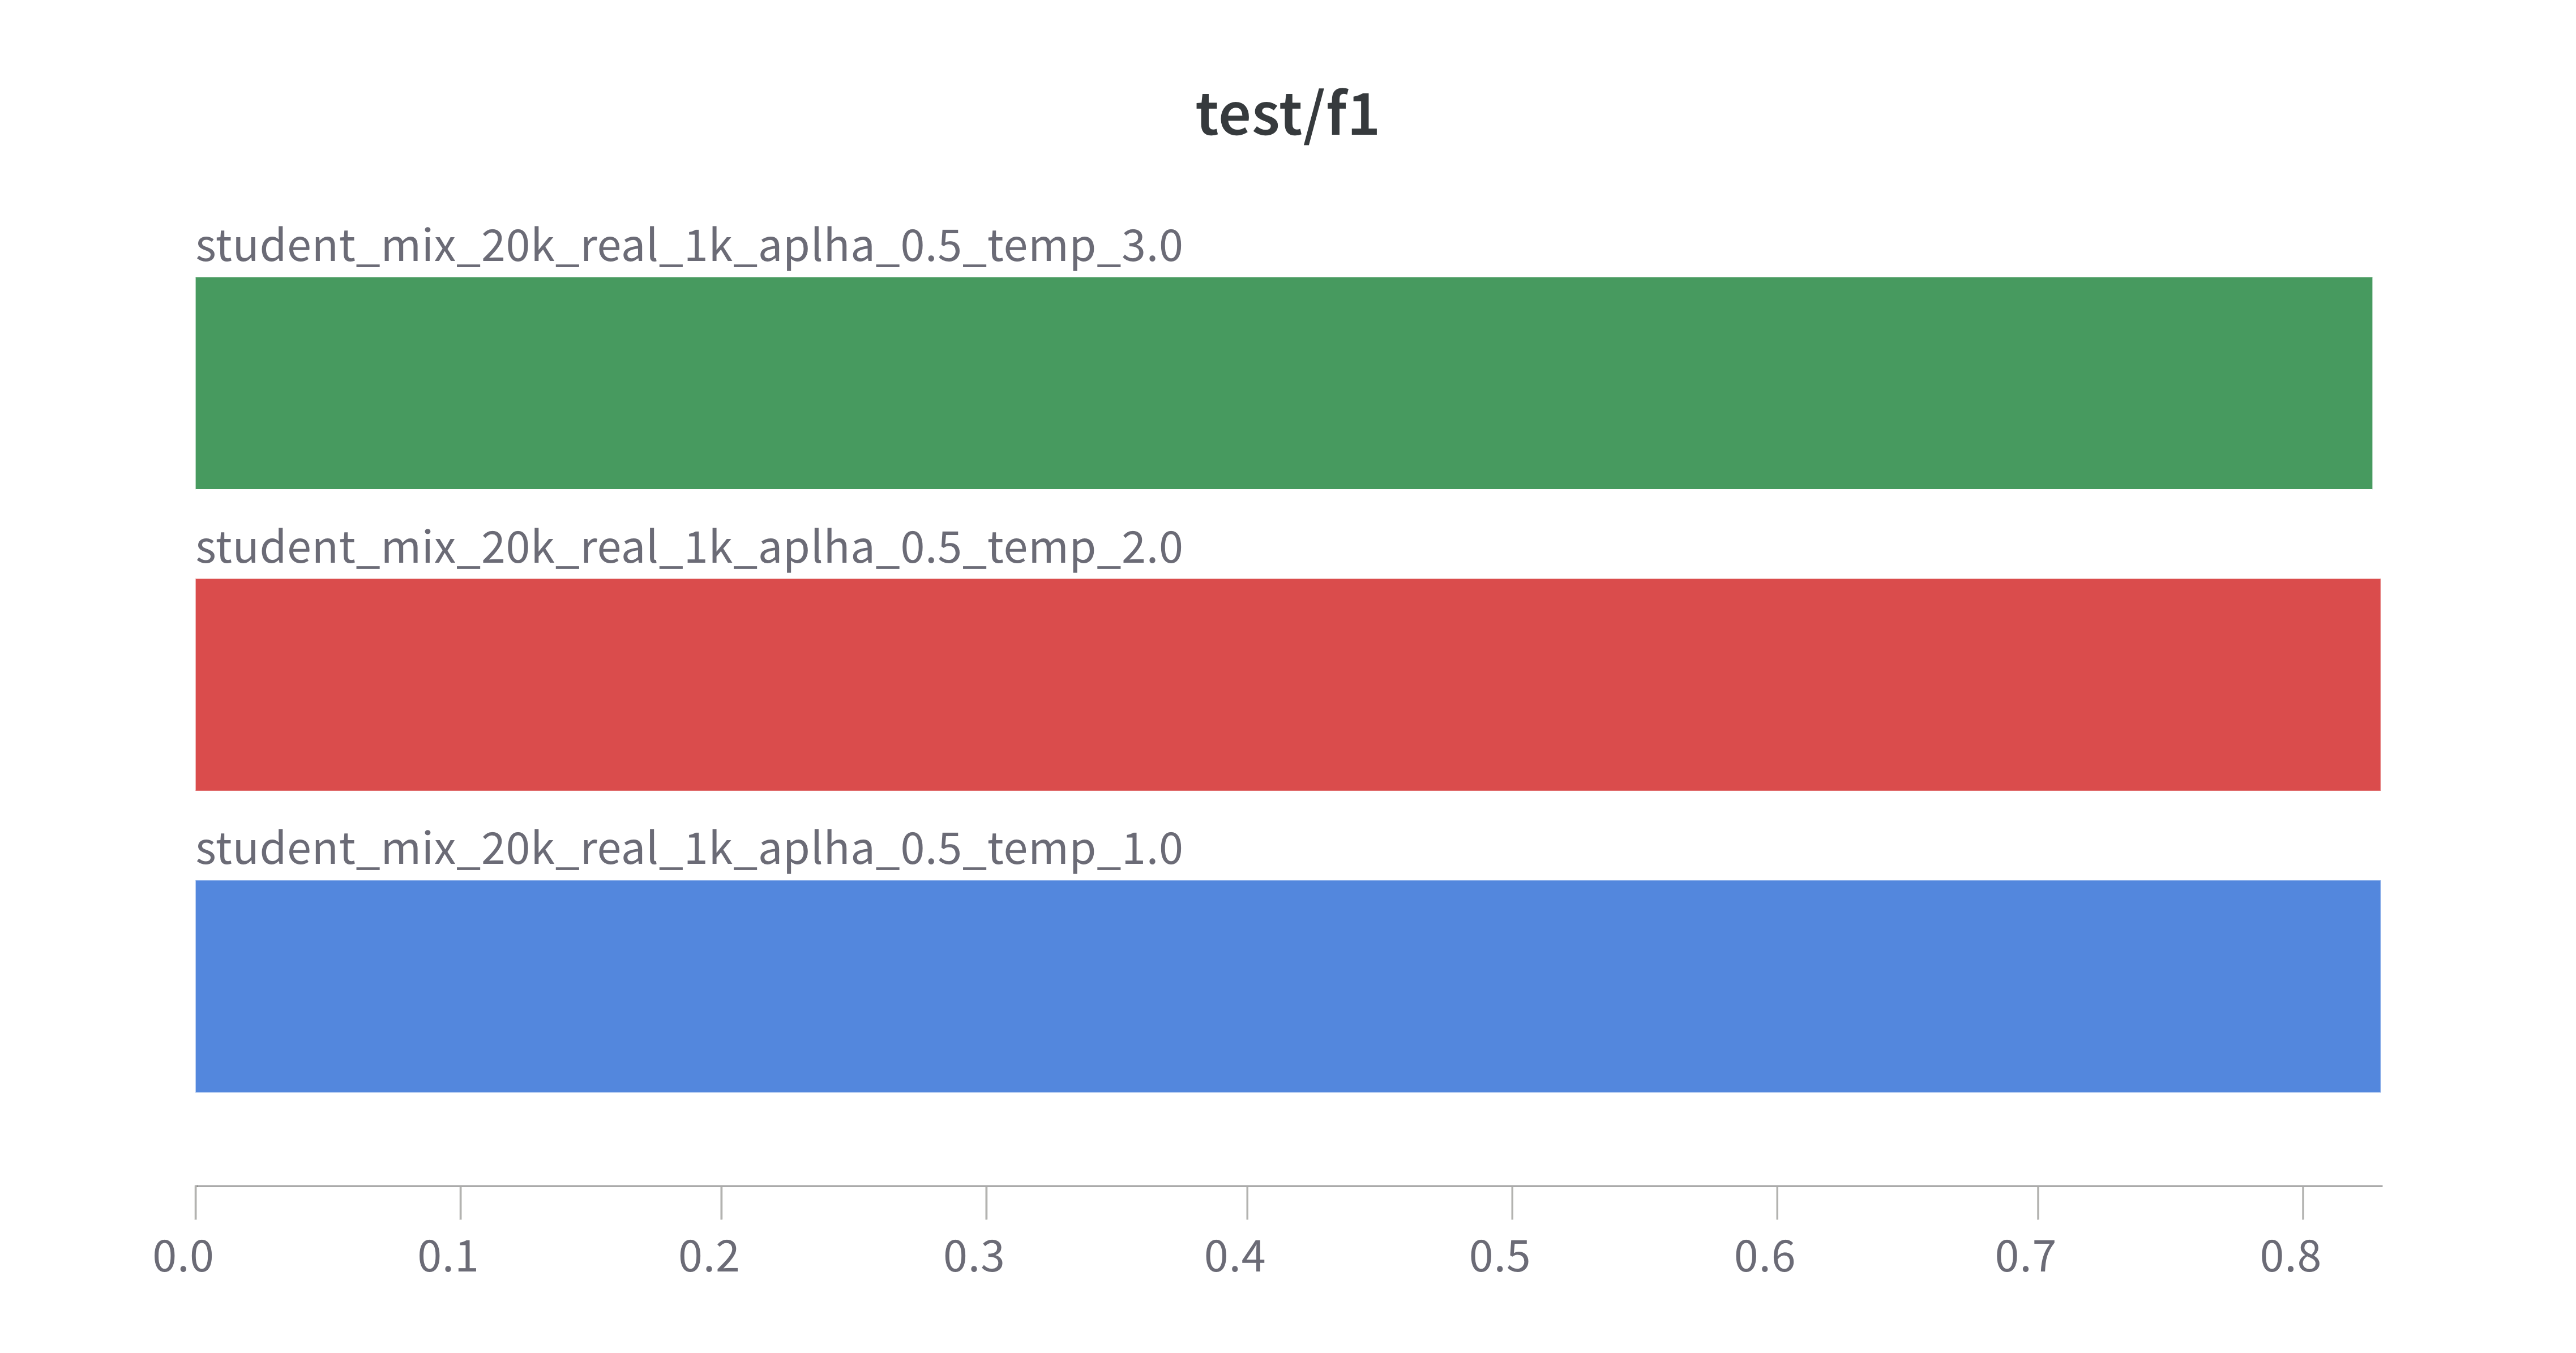
\includegraphics[width=.8\linewidth]{figures/student_temp.png}
  \caption{F$_1$ under different loss-temperature settings.}
  \label{fig:temp}
\end{figure}

\subsubsection{Effect of QC Threshold $\tau$}
\label{sec:tau}
Lowering $\tau$ to 0.7 produces the best F$_1$ even though diversity
(\emph{distinct-2}) dips slightly (Table inside
Figure~\ref{fig:tau}).  We attribute the win to richer soft-label
entropy, which outweighs the marginal diversity loss.

\paragraph{Diversity vs.\ confidence.}
Entropy of the soft labels falls from 0.681 to 0.669 as $\tau$ rises,
confirming that very strict QC collapses probabilities toward one-hot
vectors and weakens the distillation signal.  Although distinct-$n$
edges up by $\sim$1 pp at $\tau=0.9$, the information loss dominates,
hence the student performs best at $\tau=0.7$ (0.771 F$_1$).

\begin{figure}[htbp]
  \centering
  % TODO: tau sweep plot + diversity metrics
  \begin{minipage}
    {0.60\textwidth}
    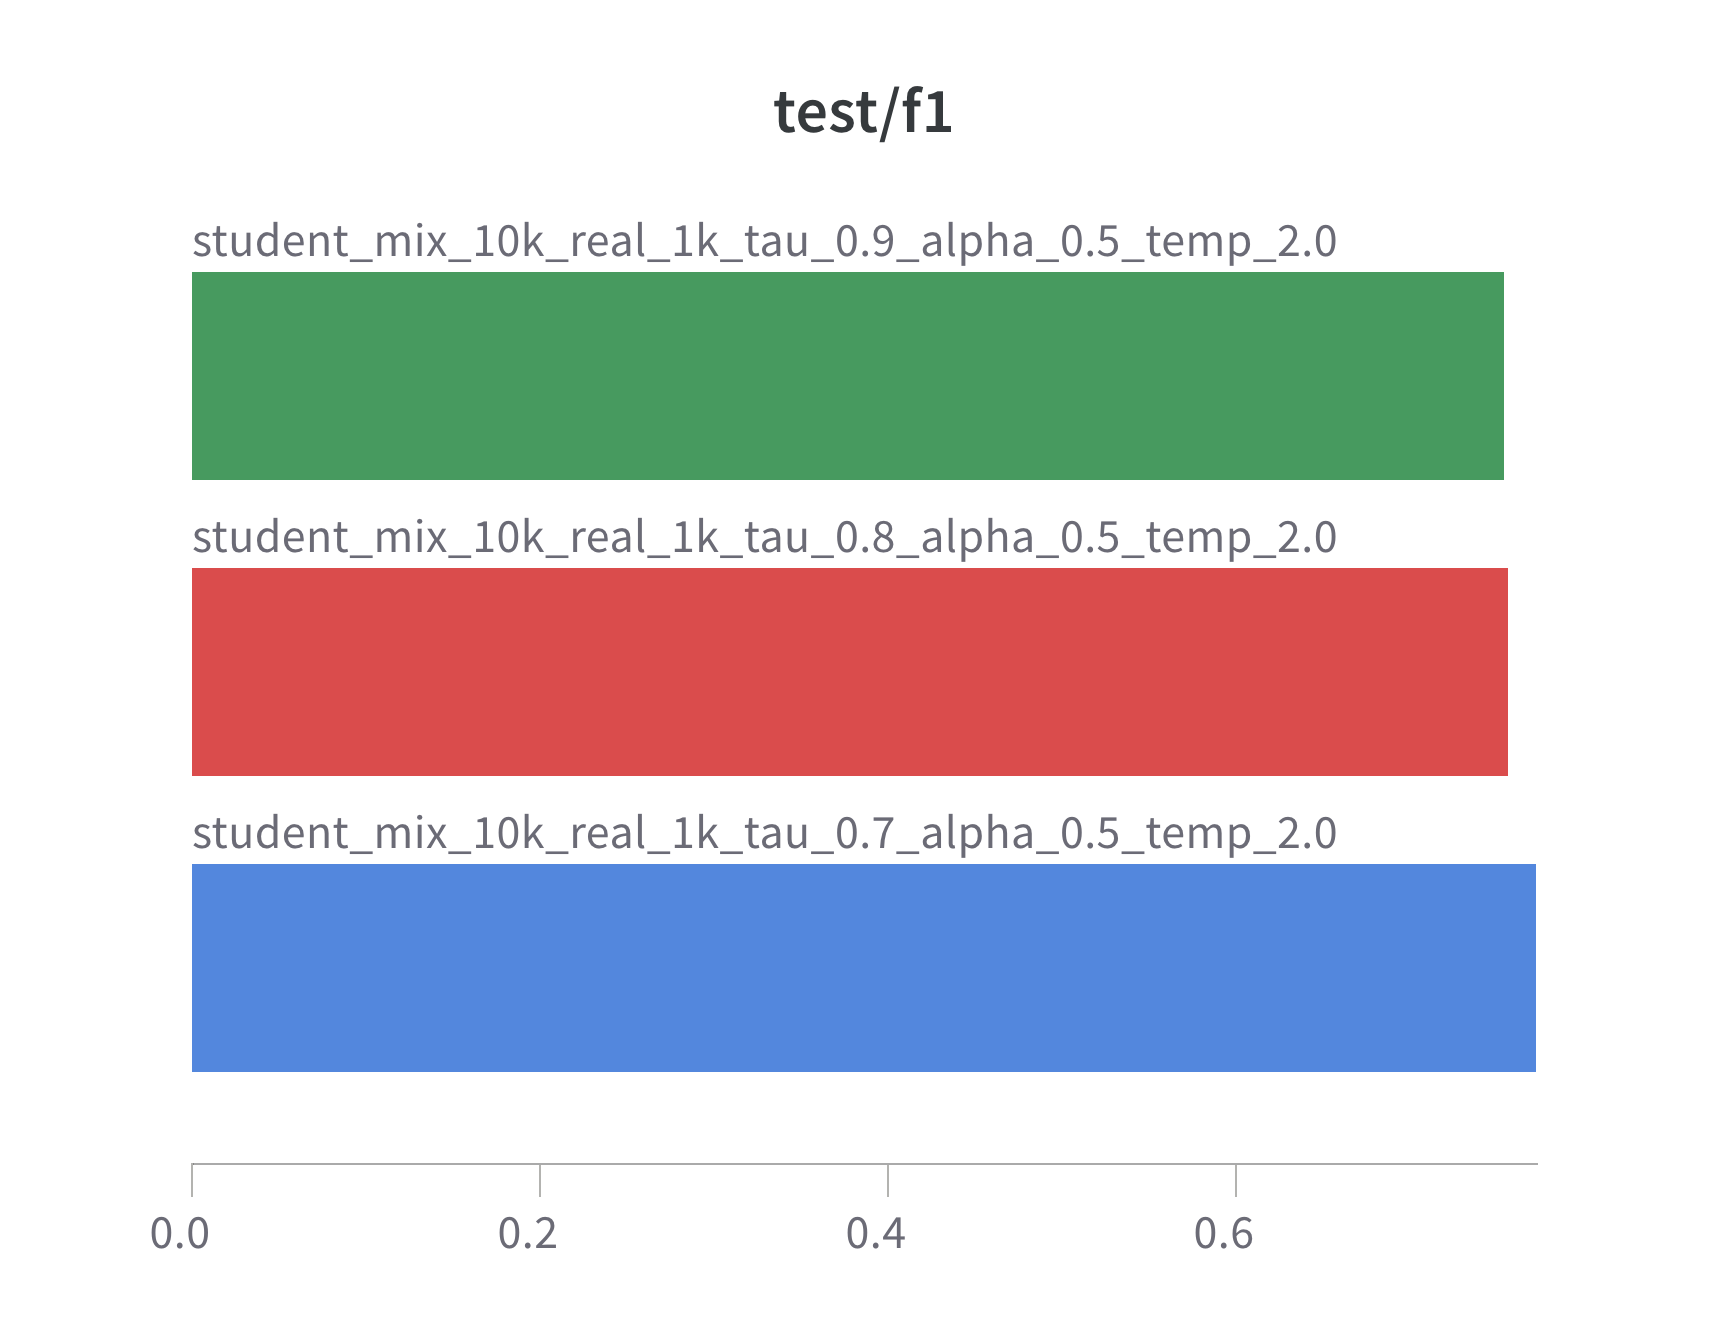
\includegraphics[width=\linewidth]{figures/student_qc_f1.png}
  \end{minipage}
  \begin{minipage}
    {0.60\textwidth}
    \centering
    \begin{tabular}{cccc}
      \toprule
      \textbf{$\tau$} & \textbf{Distinct-1} & \textbf{Distinct-2} &
      \textbf{Entropy} \\
      \midrule
      0.7 & 0.022382 & 0.262025 & 0.681052 \\
      0.8 & 0.024106 & 0.268781 & 0.675690 \\
      0.9 & 0.026319 & 0.277667 & 0.668949 \\
      \bottomrule
    \end{tabular}
  \end{minipage}
  \caption{Student F$_1$ and text-diversity as $\tau$ varies.}
  \label{fig:tau}
\end{figure}

\subsubsection{Effect of Synthetic Weight $\beta$}
\label{sec:beta}
Down-weighting synthetic rows is beneficial: $\beta=0.3$ beats
\{0.5,1.0\} by 1.8~pp on average. However, down-weighting too much
hurts performance as seen in figure~\ref{fig:beta}.
\begin{figure}[htbp]
  \centering
  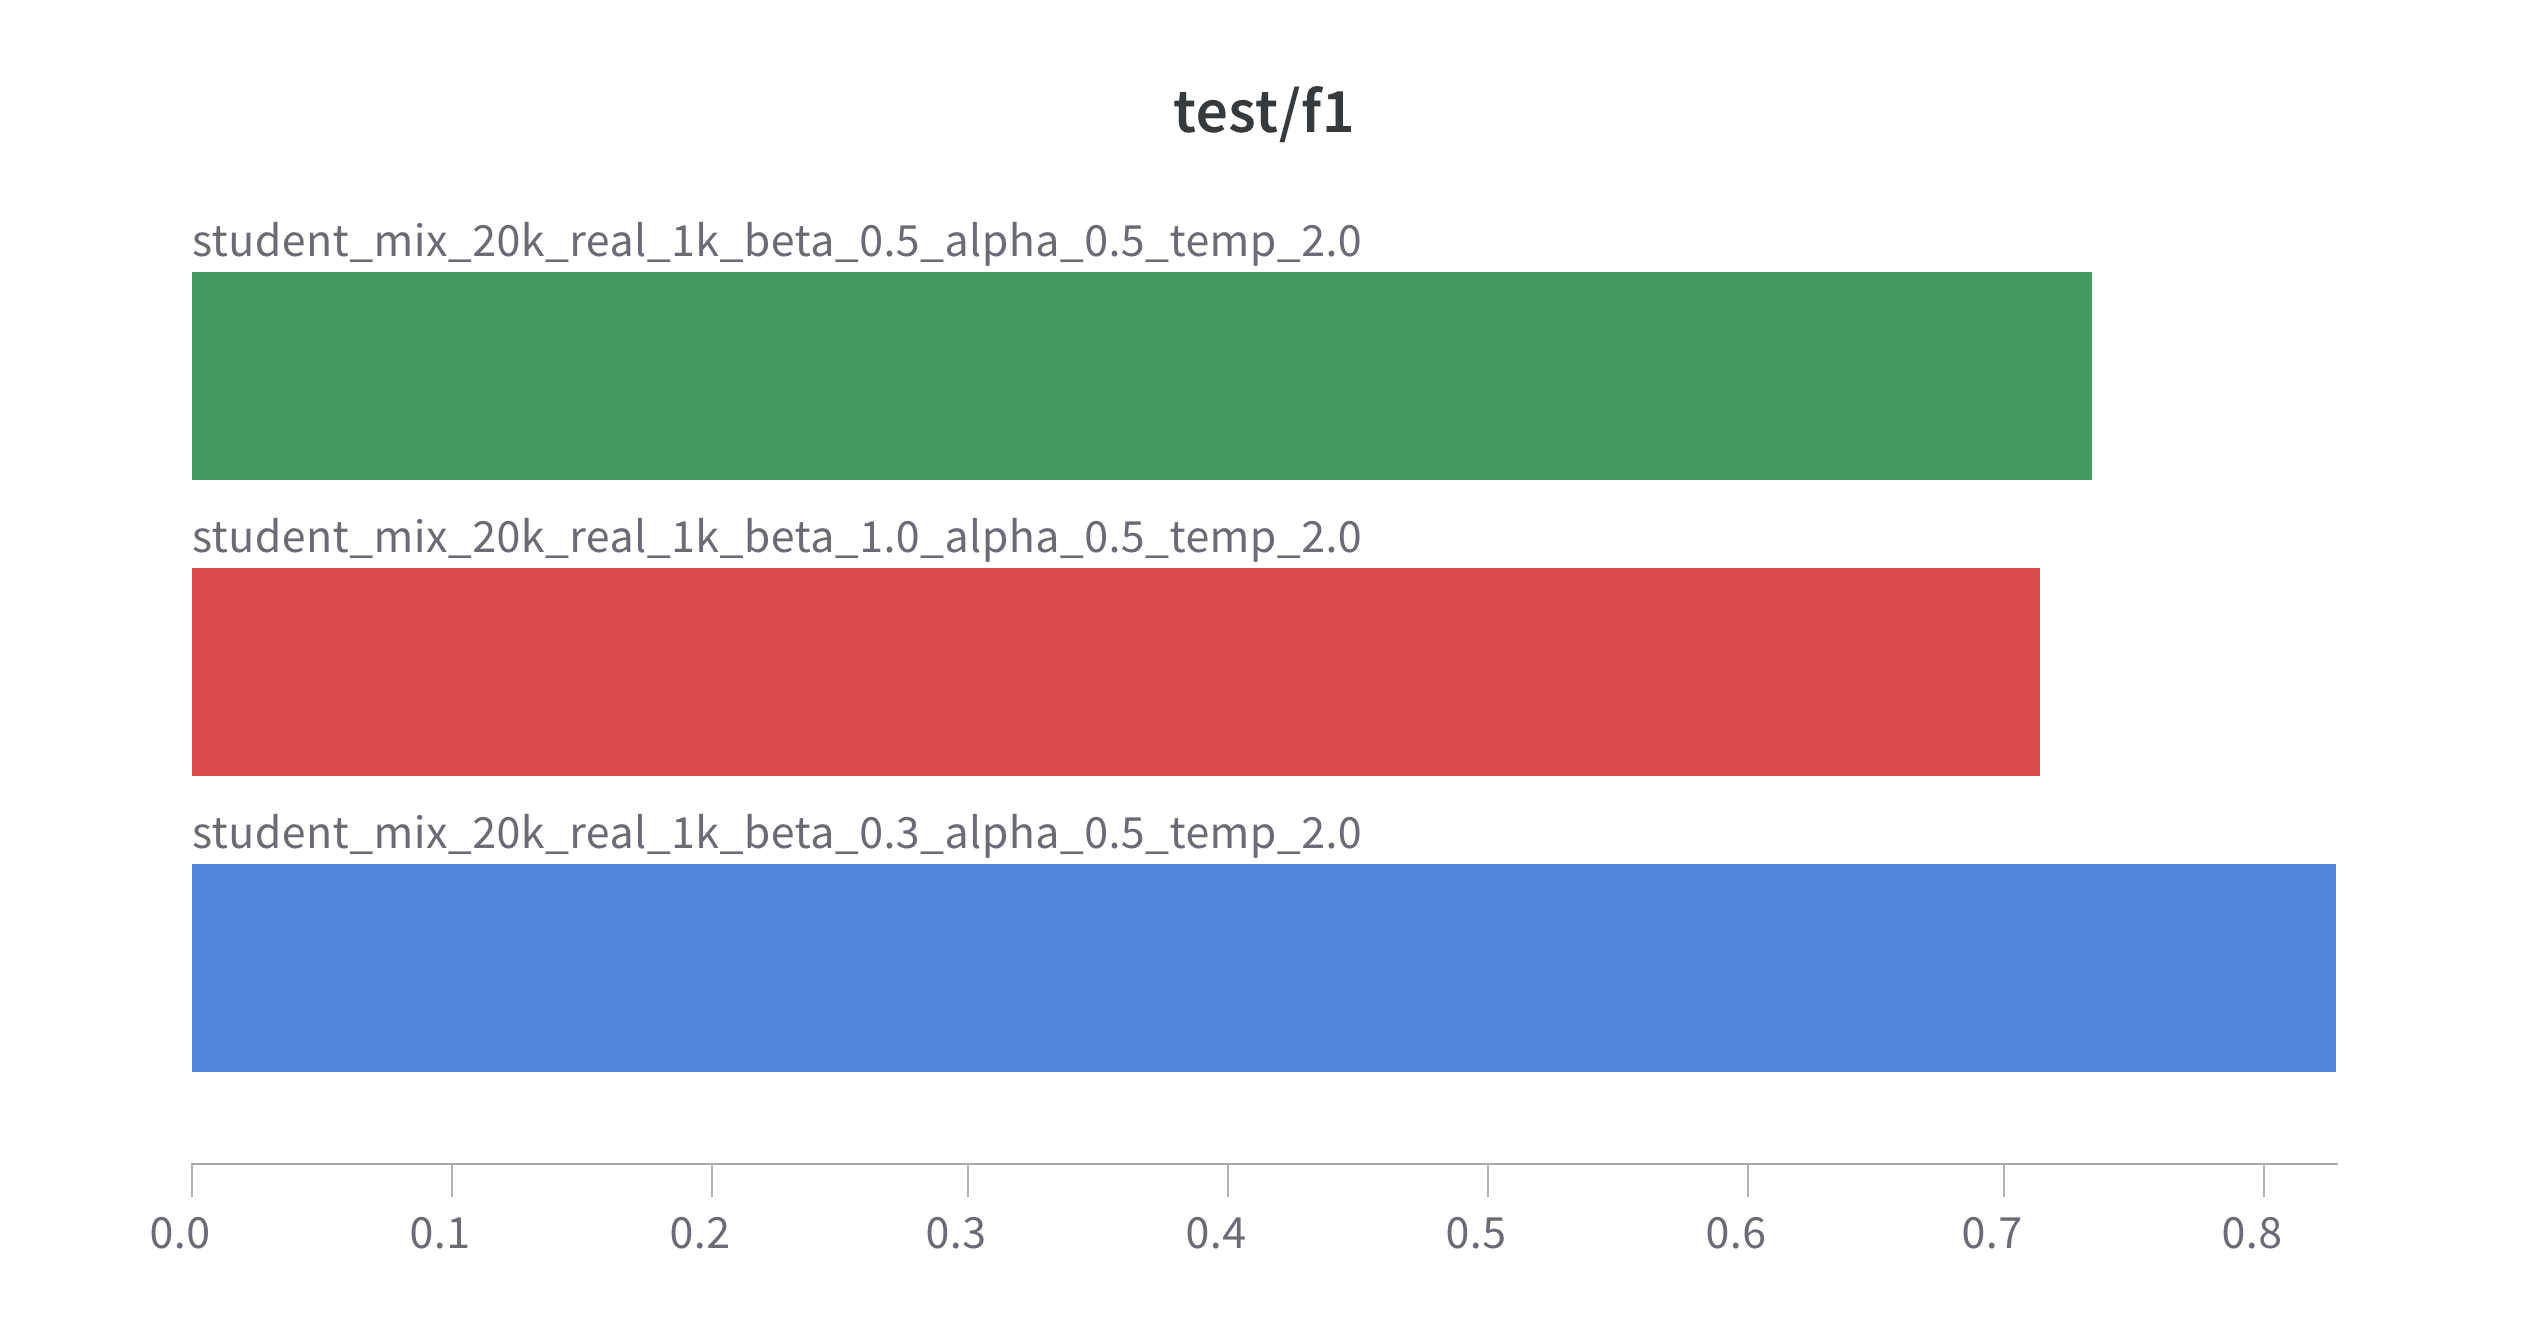
\includegraphics[width=.9\linewidth]{figures/student_beta.png}
  \caption{Performance as a function of the per-row weight $\beta$.}
  \label{fig:beta}
\end{figure}

\subsubsection{Joint Sweep: $\alpha\times\beta$}
This joint sweep study was conducted to ensure that we are using the
best combination of
$\alpha$ and $\beta$ values. The results are shown in
figure~\ref{fig:alpha-beta}. The best combination of $\alpha$ and $\beta$ is
$\alpha=0.8$ and $\beta=0.3$.

\begin{figure}[htbp]
  \centering
  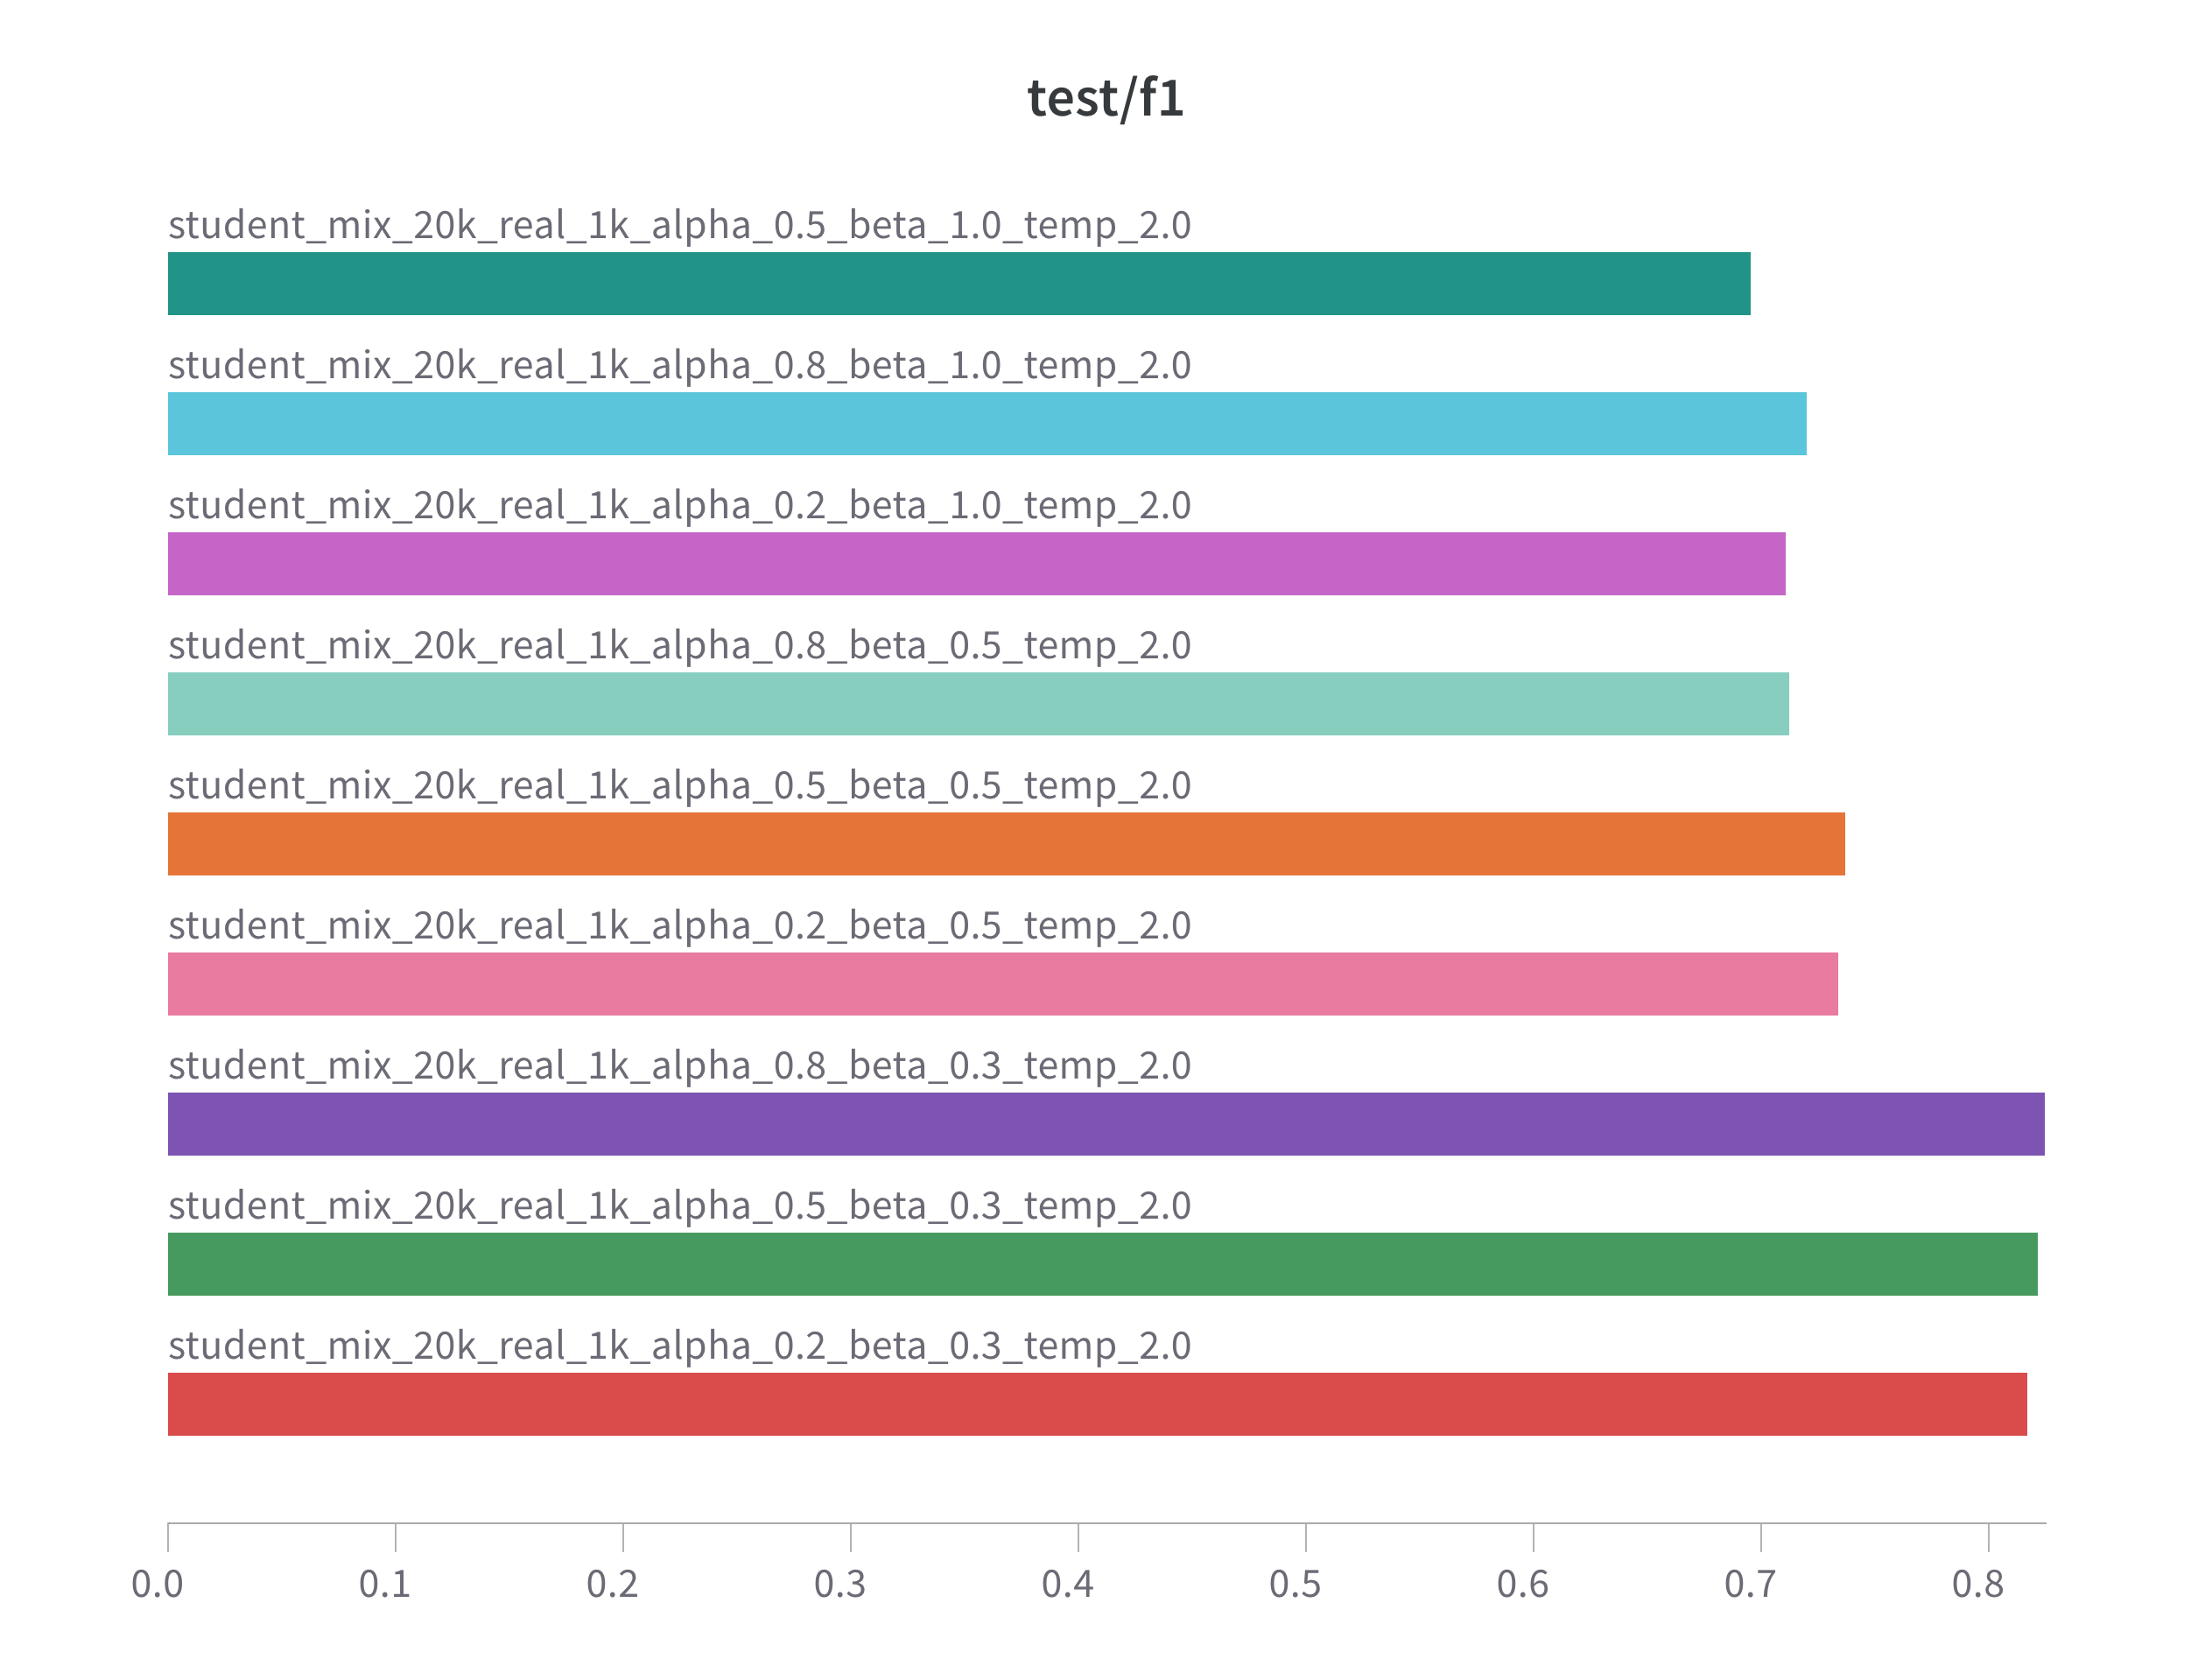
\includegraphics[width=.9\linewidth]{figures/student_alpha_beta.png}
  \caption{Performance as a function of $\alpha$ and $\beta$.}
  \label{fig:alpha-beta}
\end{figure}

% ------------------------------------------------------------------
\subsection{Error Analysis}
\label{sec:error}

\paragraph{What improved most.}
Long, negated sentences---a known weak spot for SST-2 models---saw the
largest lift.  Synthetic reviews inject new lexical cues
(\textquotedblleft did not hate\textquotedblright,
\textquotedblleft never quite worked\textquotedblright) that tighten the
decision boundary in these regions.

\paragraph{Per-class gains.}
Both classes benefit: for the 0~label (negative) precision rises
by~5 pp and recall by~6 pp, pushing macro F$_1$ from 0.79 to 0.84.

\paragraph{Remaining errors.}
Residual mistakes concentrate on sarcasm, idioms, and context-dependent
sentiment (\textquotedblleft still want my money back\textquotedblright).
Manual inspection shows that many such instances also fool the teacher,
suggesting future work on explicit sarcasm modelling or
document-level context. A sample exploration of the errors is shown
in table \ref{tab:error}.

\begin{table*}[htbp]
  \centering
  \small
  \caption{Break\-down of residual student errors by linguistic phenomenon.}
  \label{tab:error}
  \begin{tabular}{p{0.50\linewidth}ccc}
    \toprule
    \textbf{Text} & \textbf{True} & \textbf{Pred} & \textbf{Phenomenon} \\
    \midrule
    covered earlier and much better & 0 & 1 & comparative \\
    what does n\'t this film have that an impression\ldots & 1 & 0 & negation \\
    the campy results make mel brooks\ldots & 1 & 0 & intertextual reference \\
    than indecent proposal & 1 & 0 & comparative \\
    the mystery of enigma is how a rich historical\ldots & 0 & 1 & long \\
    that flow through the hollywood pipeline witho\ldots & 1 & 0 & negation \\
    it is too bad that this likable movie is n\'t more\ldots & 1 & 0
    & negation \\
    joyless & 0 & 1 & lexical brevity \\
    ready\textendash made midnight movie & 1 & 0 & idiom \\
    a third\textendash person story now, told by Hollywood,\ldots & 0
    & 1 & long \\
    nickelodeon\textendash esque kiddie flick & 1 & 0 & neologism \\
    offers no new insight & 0 & 1 & negation \\
    who needs mind\textendash bending drugs when they can see\ldots &
    1 & 0 & rhetorical question \\
    pale successor & 0 & 1 & idiom \\
    still want my money back. & 0 & 1 & sarcasm \\
    for nearly three hours & 1 & 0 & temporal \\
    amy and matthew have a bit of a phony relation\ldots & 0 & 1 & long \\
    classy & 1 & 0 & lexical brevity \\
    wo n\'t have any trouble getting kids to eat up\ldots & 1 & 0 & negation \\
    a movie with depth & 1 & 0 & idiom \\
    \bottomrule
  \end{tabular}
\end{table*}

\section{Discussion}
\label{sec:discussion}

\subsection{Impact of Teacher--Verified Synthetic Data}
The headline finding is that teacher--filtered synthetic data
closes \textasciitilde5\,pp of the performance gap between the
1\,000--row seed model and a fully supervised baseline, while requiring
one--tenth of the human annotation budget.  Ablations in
Sec.~\ref{sec:student-results} confirm that \emph{unverified} augmentation
actually hurts F$_1$ by up to 2\,pp, underlining the importance of the
verification loop.  In short, the teacher acts as a high--precision
gatekeeper, converting the raw fluency of GPT--2 into task--useful data.

\subsection{Precision--Recall Trade--offs}
Figure~\ref{fig:tau} visualises the trade--off space induced by the
confidence threshold $\tau$.  Lower $\tau$ broadens recall in the
synthetic set at the cost of precision; higher $\tau$ does the
opposite.  Interestingly the sweet spot sits at $\tau=0.7$, not the
commonly used 0.9.  We attribute this to two factors:

\begin{enumerate}
  \item higher entropy in the teacher logits, which gives the student
    richer gradient information,
  \item diminishing returns from the marginal gain in label purity
    above 0.8.
\end{enumerate}

\subsection{Quality--Control Effectiveness}
The three filters in Stage~C (teacher check, length, ASCII printable)
reject 32\,\% of the raw generations.  Manual inspection of
100 rejects finds that 74 fall into obvious error categories
(e.g.\ sentiment drift, malformed tokens), suggesting the QC
pipeline is removing genuine noise rather than useful diversity.
Moreover, distinct--2 increases marginally with stricter $\tau$, so
diversity does not suffer from verification per~se but from the
entropy collapse that accompanies very high confidence levels.

\subsection{Limitations}
\begin{itemize}
  \item \textbf{Single dataset.}  All experiments use SST--2; transfer to
    other domains or multilingual settings is untested.
  \item \textbf{Teacher reliability.}  The teacher is fine--tuned on only
    1\,k rows.  Its own biases propagate into both the synthetic set
    and the student.
  \item \textbf{Compute cost.}  Although the student is small, generating
    20\,k verified sentences takes significant compute.
  \item \textbf{Qualitative pruning.}  The switch from the
    lowest--perplexity
    generator to a higher--perplexity but cleaner checkpoint relies
    on human judgement rather than an automatic metric.
\end{itemize}

\subsection{Ethical Considerations and Bias Analysis}
Synthetic text can amplify the biases of both the generator and the
teacher.  While the
teacher filter reduces outright label noise, it does not neutralise
sensitive attributes embedded in the generator's training data.
We therefore recommend:

\begin{enumerate}
  \item inserting a lightweight toxicity/bias classifier into
    Stage~C,
  \item auditing the synthetic corpus with crowd workers,
  \item releasing all checkpoints under a license that discourages
    sensitive downstream use without further debiasing.
\end{enumerate}

\vspace{1em}
\section{Future Work}
\label{sec:future}

\begin{enumerate}
  \item \textbf{Sarcasm and context.}
    Integrate a discourse--level module or contrastive prompts to
    handle ironic sentiment that both teacher and student miss.
  \item \textbf{Adaptive $\tau$.}
    Replace the static threshold with a
    bandit that maximises downstream dev F$_1$ on--the--fly.
  \item \textbf{Active learning.}
    Show the lowest--confidence synthetic sentences to a human
    annotator; combine human feedback with the KD loss.
  \item \textbf{Cross--lingual transfer.}
    Prompt a multilingual generator (e.g.\ mGPT) and use a
    cross--lingual teacher to bootstrap low--resource languages.
  \item \textbf{Fairness diagnostics.}
    Couple the pipeline with differential privacy or
    counterfactual fairness metrics to monitor bias drift as more
    synthetic data is added.
\end{enumerate}

\vspace{1em}
\section{Conclusion}
\label{sec:conclusion}

SentiSynth demonstrates that a tight
\emph{generate $\rightarrow$ verify $\rightarrow$ distil} loop can
deliver better sentiment classification with only
1\,000 human labels.  Key to this success is the synergy between
teacher verification, soft--label distillation, and judicious
re--weighting of synthetic rows.  While limitations remain
(single--domain evaluation, potential bias transfer), the framework is
modular: stronger teachers or smarter generators can be plugged in
with minimal code changes.

\appendix
\section{Appendix}
\section{Repository Structure}
\label{sec:appendix-structure}
\noindent\textbf{Top-level layout (selected)}
\begin{verbatim}
configs/                experiment hyper-parameters
|
+-- generator/          GPT-2 fine-tuning configs
|   +-- sst2_hf.yaml
+-- student/            DistilBERT KD configs
|   +-- real_1k.yaml
|   +-- student_mix.yaml
+-- synthetic/          synthetic-dataset generation
|   +-- conf.yaml
+-- teacher/            DeBERTa fine-tuning configs
    +-- deberta_large_sst2_mps.yaml
    +-- sst2_hf.yaml
\end{verbatim}

\begin{verbatim}
src/                    project source code
|
+-- cli/                end-to-end command-line pipelines
|   +-- 01_train_teacher.py
|   +-- 02_fine_tune_generator.py
|   +-- 03_create_synthetic_dataset.py
|   +-- 04_build_student_datasets.py
|   +-- 05_train_student.py
|
+-- training/           custom Trainer subclasses
|   +-- student_weighted_soft_trainer.py
|
+-- utils/              helpers (metrics, prompts, wandb)
|   +-- metrics.py
|   +-- prompts.py
|   +-- wandb_setup.py
|
+-- data.py             shared dataset utilities
+-- models.py           model builder functions
+-- nb.py               notebook helper for quick sampling
\end{verbatim}

\noindent\textbf{Reproducibility shortcuts}
\begin{verbatim}
python src/cli/01_train_teacher.py        configs/teacher/sst2_hf.yaml
python src/cli/02_fine_tune_generator.py  configs/generator/sst2_hf.yaml
python src/cli/03_create_synthetic_dataset.py  configs/synthetic/conf.yaml
python src/cli/04_build_student_datasets.py    ...
python src/cli/05_train_student.py        configs/student/student_mix.yaml
\end{verbatim}

\noindent
See the YAML files under \texttt{configs/} for per-stage
hyper-parameters and output paths.

\section{Example Dataset Shape}
When we generate the synthetic dataset, we save it in a JSONL format.
This is an example of what it looks like:
\begin{verbatim}
==================================================
First 10 samples of train:
==================================================

#    Text                                               Label
---- -------------------------------------------------- ------
1    a must read for anyone who about to bolt the theat 1
2    a compelling story with lots of intrigue suspense  1
3    one of the best in recent memory latest film and i 1
4    the movie is too long and dull it like trying to m 0
5    a half hour long plot is flat with nothing new to  0
6    the film characters and their actions are so detai 0
7    the film star is n't very bright but it does its b 1
8    an exhilarating documentary that has you in the dr 1
9    a film so bad it not even funny '' i mean if you w 0

 Soft Labels                              Weight  is_Synth
---------------------------------------- -------- -----
[0.3782115876674652, 0.6217884421348572]  0.30     1
[0.37769943475723267, 0.6223005652427673] 0.30     1
[0.37762364745140076, 0.6223763227462769] 0.30     1
[0.6219679713249207, 0.37803205847740173] 0.30     1
[0.622056245803833, 0.37794366478919983]  0.30     1
[0.6173325777053833, 0.3826673924922943]  0.30     1
[0.37869372963905334, 0.621306300163269]  0.30     1
[0.37759384512901306, 0.6224061250686646] 0.30     1
[0.6220729947090149, 0.3779270350933075]  0.30     1

\end{verbatim}

\section{Full Metrics Logs}
The full metrics logs for the teacher, generator and student models
are available at the following
weights and biases links:
\begin{itemize}
  \item \url{https://api.wandb.ai/links/paramkpr-reed-college/1x1fwy5w}
  \item \url{https://api.wandb.ai/links/paramkpr-reed-college/4dk0u510}
  \item \url{https://api.wandb.ai/links/paramkpr-reed-college/xzxetj1g}
  \item \url{https://api.wandb.ai/links/paramkpr-reed-college/0qq2jnh3}
  \item \url{https://api.wandb.ai/links/paramkpr-reed-college/ynsp9i59}
  \item \url{https://api.wandb.ai/links/paramkpr-reed-college/w5i5m8gj}
\end{itemize}

% ----------------------------------------------------------------------
\newpage
\bibliographystyle{plain}
\bibliography{refs}
\end{document}
